\documentclass[12pt]{article}
% preamble.tex

% enclose any latex in \comment{} to suppress it
\newcommand{\comment}[1]{}
\newcommand{\citeNP}[1]{\cite{#1}}

\usepackage{graphicx}
\usepackage{multicol}
\usepackage{times}
\usepackage{floatflt}
\graphicspath{{./}{figures/}}

% NO psfig -- pdflatex does not support it ...
% \usepackage{psfig}
% \psfigurepath{./:figures/}
% \DeclareGraphicsRule{.eps.gz}{eps}{.eps.bb}{'gunzip -c #1}

\newcommand{\upline}{\vspace*{-\baselineskip}}
\newcommand{\up}{\vspace*{-6pt}}
\newcommand{\downline}{\vspace*{\baselineskip}}
\newcommand{\sep}{~~~~~~~~~~}

% this hardcodes the bib name, which we don't want to do.
% \renewcommand{\thebibliography}[1]{\section*{References Cited}
% \addcontentsline{toc}{section}{References Cited}\list
%  {[\arabic{enumi}]}{\settowidth\labelwidth{[#1]}\leftmargin\labelwidth
%  \advance\leftmargin\labelsep
%  \usecounter{enumi}}
%  \def\newblock{\hskip .11em plus .33em minus -.07em}
%  \sloppy\clubpenalty4000\widowpenalty4000
%  \sfcode`\.=1000\relax}

% fix this to specify width and height, and solve for the margins
% margins.tex

% import calc
\usepackage{calc}

%
\newlength{\myrightmargin}
\newlength{\myleftmargin}
\newlength{\mytopmargin}
\newlength{\mybottommargin}

% Change these settings to change the margins
\setlength{\myrightmargin}{1.0in}
\setlength{\myleftmargin}{1.0in}
\setlength{\mytopmargin}{0.75in}     
\setlength{\mybottommargin}{0.75in} 
\setlength{\oddsidemargin}{0.0in}   % extra room on inside side

%%% use margin settings to set width variables
\setlength{\evensidemargin}{0 in}
\setlength{\marginparsep}{0 in}
\setlength{\marginparwidth}{0 in}
\setlength{\hoffset}{\myleftmargin - 1.0in}
\setlength{\textwidth}
  {8.5in -\myleftmargin -\myrightmargin -\oddsidemargin}

%%% use margin settings to set height variables
\setlength{\voffset}{\mytopmargin -1.0in}
\setlength{\topmargin}{0 in}
\setlength{\headheight}{12 pt}
\setlength{\headsep}{20 pt}
\setlength{\footskip}{36 pt}
\setlength{\textheight}
  {11.0in-\mytopmargin-\mybottommargin-\headheight-\headsep-\footskip}

% \oddsidemargin 0.2cm
% \evensidemargin 0cm
% \textwidth 16.0cm
% \topmargin -1.25cm
% \textheight 22.94cm

% remove parindent, squeeze grafs
\setlength{\parindent}{0in}
\setlength{\parskip}{1ex}

\def\nibf#1{\noindent\textbf{#1}}


\usepackage{hyperref}
%\usepackage[hyperpageref]{backref}

\usepackage[]{caption}
\setlength{\abovecaptionskip}{0pt}
\setlength{\belowcaptionskip}{-5pt}
\setlength{\intextsep}{10pt plus 2pt minus 2pt}


\usepackage{wrapfig}
\usepackage{paralist}
\usepackage{amsmath}
\usepackage{amssymb}
\usepackage{amsfonts}
\usepackage{textcomp}
\usepackage{subfig}
\usepackage{framed}
\usepackage{setspace}
\usepackage{here}
\usepackage[numbers, square, comma, sort&compress]{natbib}
\usepackage[compact]{titlesec}
\titlespacing{\section}{0pt}{0ex}{0pt}
\usepackage{color}
%\usepackage{SIunits}

\newenvironment{packed_enum}{
\begin{enumerate}
  \setlength{\topsep}{0pt}
  \setlength{\partopsep}{0pt}
  \setlength{\itemsep}{1pt}
  \setlength{\parskip}{0pt}
  \setlength{\parsep}{0pt}
}{\end{enumerate}}

\newcommand{\blue}[1]{\textcolor{blue}{#1}}

\usepackage{float}
\floatstyle{plaintop}
\newfloat{program}{thp}{lop}
\floatname{program}{Table}
%\setlength{\intextsep}{10pt plus 2pt minus 2pt}
% bold face: highlight keywords, or big ideas
% italics: inconspicuous stressing of key points
% underline: hypothesis; avoid

\usepackage{bm}

\date{\today }
\title{LAMP-solar}

\begin{document}

\setcounter{page}{1}

\maketitle
%\newpage
\pagenumbering{roman}
%\newpage
\pagestyle{empty}

\tableofcontents
\newpage
\listoffigures
%\listoftables
\listof{program}{List of Tables}

\newpage
\pagestyle{plain}
\setcounter{page}{1}
\pagenumbering{arabic}

\section{Solar Spectrum}

The solar spectrum data is found in ASTMG173.txt as obtained from \cite{SolarAM15}.
This contains 
\begin{itemize}
\item AM0: Outer space ($1,366$ W/m$^2$),
\item AM1.5 Global: Used for testing Flat panels ($1,000$ W/m$^2$), and 
\item AM1.5 Direct: Used for testing of concentrators ($900$ W/m$^2$).
\end{itemize}

\begin{figure}[H]
\centering
\vspace{-10pt}
 \subfloat[]{\label{fig:IrradianceVersusWavelength}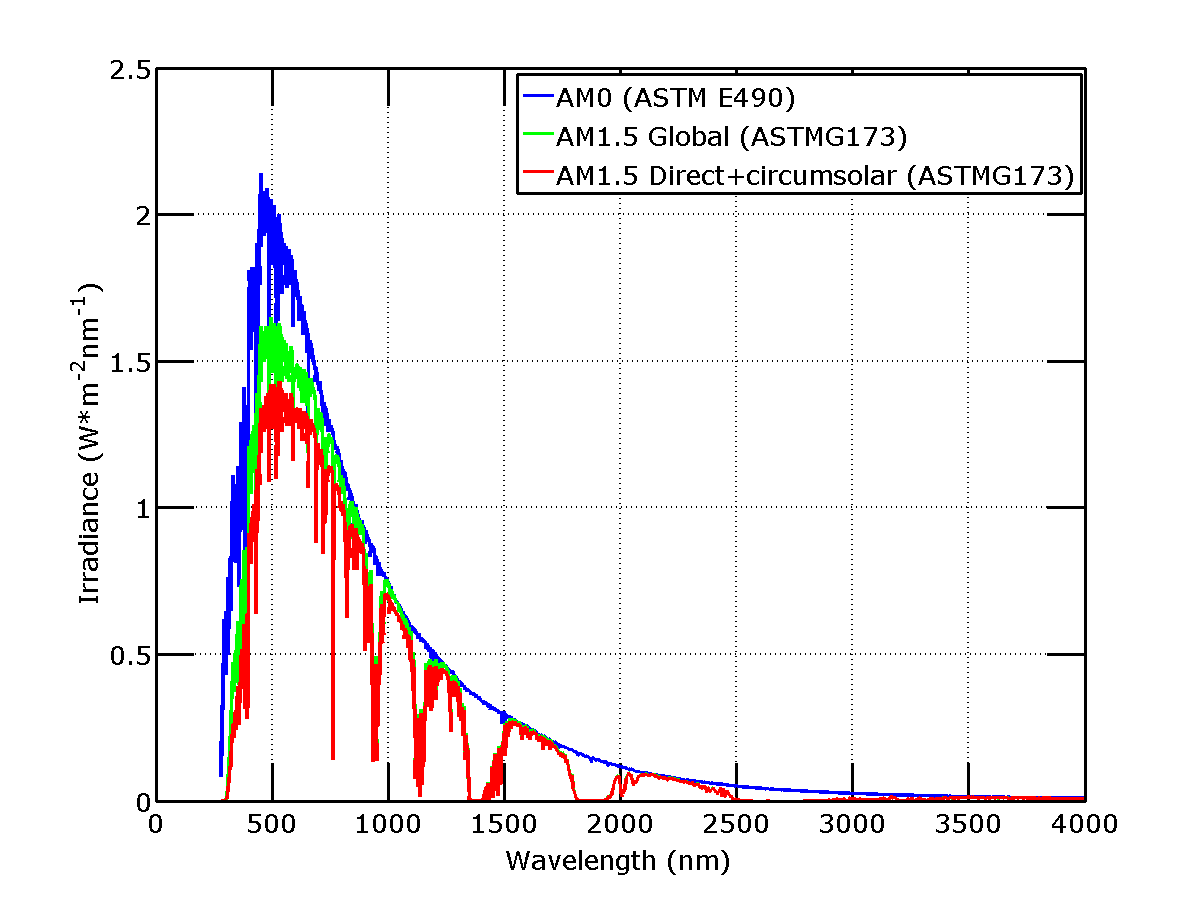
\includegraphics[width=0.45\textwidth]{Figures/IrradianceVersusWavelength}}
 \hspace{5pt}
 \subfloat[]{\label{fig:IrradianceVersusEnergy}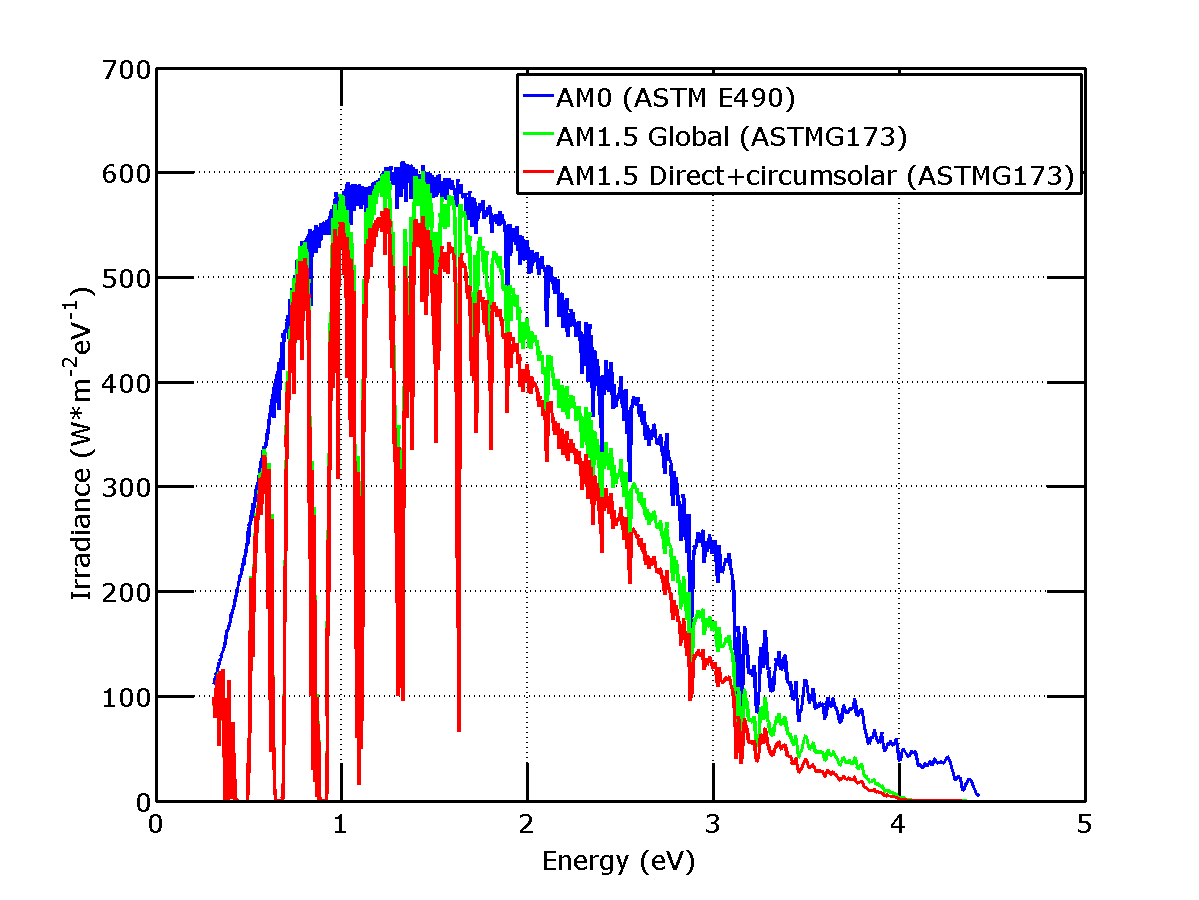
\includegraphics[width=0.45\textwidth]{Figures/IrradianceVersusEnergy}} 
 \caption[Solar Spectrum]{Solar Spectrum}
  \label{fig:SolarSpectrum}
\end{figure}

The sun has a temperature of about 5760 K and emission is strongest in the visible wavelengths between $390$ and $750$ nm.  The emitted photon flux density per unit area per unit solid angle per unit frequency which is derived later on from the Bose-Einstein Distribution and the density of states is 
\begin{equation}
b_\Omega(E) dE d\Omega = \frac{2 n^2}{h^3 c^2} \frac{E^2}{\exp{(\frac{E - \mu}{k T}}) -1} dE d\Omega
\end{equation}

Viewed from the Earth, the sun has an angular diameter of 32$^{\prime}$ or 0.53$^{\circ}$.  Thus, 
\begin{equation}
\int_0^{2 \pi} \int^{\frac{0.53 \times \pi}{180}}_0 b_\Omega(E) \cos \theta \sin \theta d\theta d\phi = 2.166 \times 10^{-5} \pi  b_\Omega(E)
\end{equation}
for radiation from the sun.  

\begin{figure}[H]
\centering
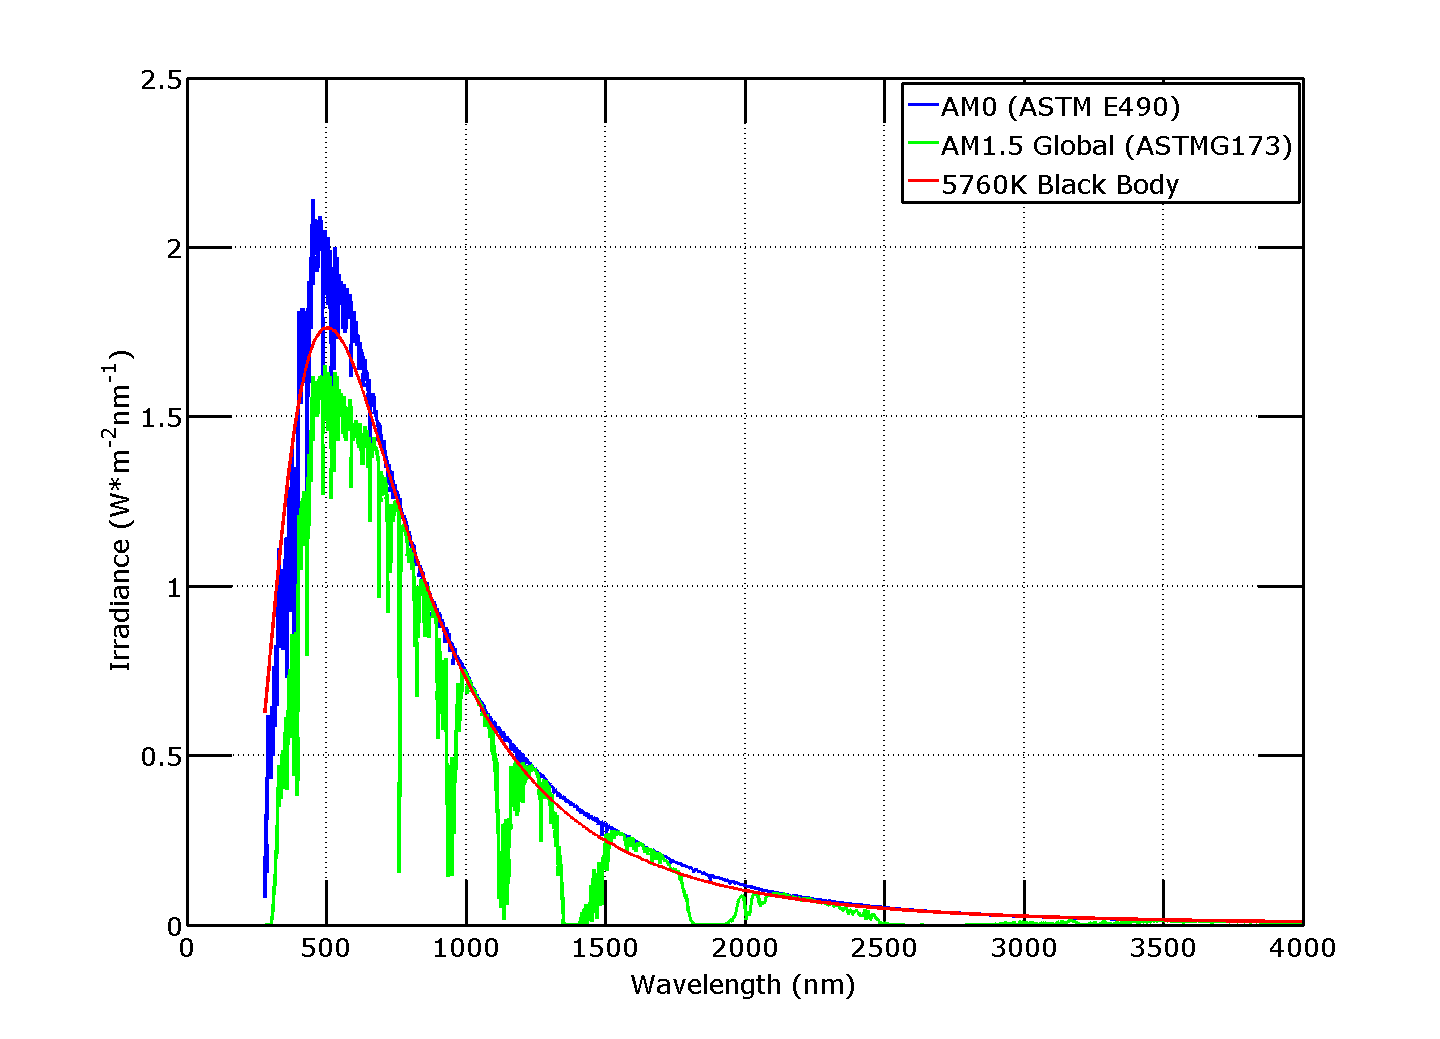
\includegraphics[width=0.45\textwidth]{Figures/IrradianceVersusWavelengthWithBlackbody}
 \caption[Solar Spectrum with 5760 K black body]{Extra-terrestrial (Air Mass 0) solar spectrum compared with 5760 K black body spectrum reduced by a factor of $4.6 \times 10^4$ and with the standard terrestrial (Air Mass 1.5) spectrum.}
  \label{fig:SolarSpectrumwBlackBody}
\end{figure}


\begin{equation}
\boxed{I(E) = E b_s(E)}
\end{equation}
where $b_s(E)$ is the photon flux density and $I(E)$ is the irradiance or power flux density.
$\int_0^{\infty} I(E) dE = 1,000$ W/m$^2$ for AM1.5 Global.  

The distance $d$ that light travels through the atmosphere of thickness $d_0$ from the sun incident at an angle $\alpha$ is 
\begin{equation}
\boxed{d = \frac{d_0}{\cos \alpha}}
\end{equation}
The ratio $d/d_0$ or $1/\cos \alpha$ is called the air-mass coefficient.  
The spectrum outside the atmosphere is designated by AM0 and the typical spectrum for moderate climates such as the contiguous United State is AM1.5, which corresponds to the angle of incident of solar radiation, $\alpha = 48^{\circ}$.

The relationship between frequency $\nu$ (in Hz or 1/sec), angular frequency $\omega$ (with units of radians per second; $\omega = 2 \pi \nu$), wavelength $\lambda$, and energy $E$ of light is
\begin{equation}
\boxed{E = h \nu =  \hbar \omega} \label{eq:energy}
\end{equation}
where $h$ is the Planck constant and $\hbar$ is the reduced Planck constant ($\hbar = \frac{h}{2 \pi}$).
\begin{equation} 
\boxed{E/eV = 1240/(\lambda/nm)}
\end{equation}

The phase velocity is defined as 
\begin{equation}
\boxed{v_p = \frac{\omega}{k}} \label{eq:phaseVelocity}
\end{equation}
where $k$ is the wavenumber of the magnitude of the wave vector $\mathbf{k}$.  

The wavelength, or spatial variation between neighboring field peaks, is related to frequency by 
\begin{equation}
\boxed{\lambda = \frac{v_p}{\nu} = \frac{2 \pi}{k} n}
\end{equation}
where $v_p$ is the phase speed.  %The prime indicates the wavelength of light inside a medium.  $\lambda$ is the wavelength of light in a vacuum.  
In vacuum, $v_p = c = 3 \times 10^8$ m/sec, the speed of light.  
\begin{equation}
\boxed{v_p = \frac{c}{n}} \label{eq:phaseVelocity2}
\end{equation}
 in other media where $n$ is the index of refraction and a function of frequency.      
%$E = p v_p$



The momentum is 
\begin{equation}
\boxed{p = \hbar k= \frac{h}{\lambda}}
\end{equation}
%where $k$ is the wavenumber.  
%$p = \frac{h \nu}{v_p} = \frac{h}{\lambda}$
The wavenumber (sometimes referred to as the angular wavenumber) is defined as 
\begin{equation}
\boxed{k = \frac{2 \pi}{\lambda} n}
\end{equation}

\subsection{Optical Properties}

The integrated absorption, reflection, and transmission may be calculated from 
\begin{equation}
A_i = \frac{\int b_s(E) A(E) dE}{\int b_s(E) dE} 
\end{equation}
where $A_i$ is the integrated absorption, and $A(E)$ is the absorption as a function of E.  



\section{Ultimate Efficiency}

The ultimate efficiency is defined as
\begin{equation}
\boxed{\eta_{ue} = \frac{\int_{0}^{\lambda_g} I(\lambda) A(\lambda) \frac{\lambda}{\lambda_g} d\lambda}{\int_{0}^{\infty} I(\lambda) d\lambda} = \frac{\int_{E_g}^{\infty} I(E) A(E) \frac{E_g}{E} dE}{\int_{0}^{\infty} I(E) dE} }
\end{equation}
where $E_g$ is the band gap and $\lambda_g$ is the wavelength corresponding to the band gap and $A(\lambda$) or $A(E)$ is the absorption at a particular wavelength or energy.  Ultimate efficiency assumes that the temperature of the cell $T_c = 0$ K such that there is no recombination.   

The solar cell is assumed to be perfectly absorbing, non-reflecting material such that the (external) quantum efficiency is
\begin{equation}
QE(E) = A(E) = \begin{cases} 
1, E \geq E_g\\ 
0, E < E_g \end{cases}.
\end{equation}
Each photon with energy greater than the band gap produces one electron-hole pair, and these carriers are collected without recombination.    

\begin{figure}[H]
\centering
 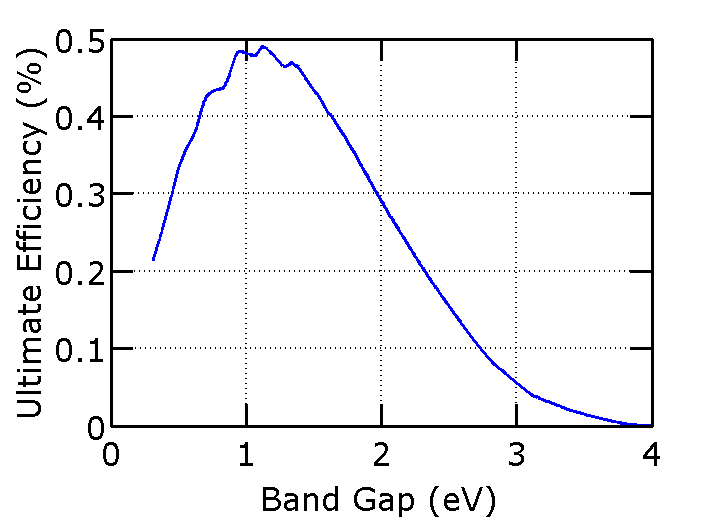
\includegraphics[scale=.4]{Figures/UltimateEfficiencyVersusEnergy}
 \caption{Ultimate Efficiency versus Band gap energy}
  \label{fig:leadingThermoelectrics}
\end{figure}

\section{Limiting Efficiency}

The limiting efficiency considers radiative recombination of electron-hole pairs through spontaneous emission.  
This detailed balance limit of efficiency is also referred to as the \textbf{Shockley-Queisser efficiency} \cite{Shockley:61}.  

All matter with temperature greater than 0 K continuously emits \textbf{thermal radiation}.  The solar cell emits electromagnetic radiation due to its temperature while absorbing radiation incident on it from the surrounding environment due to its temperature.  The rate of photon emission and absorption are balanced according to \textbf{detailed balance}, $\epsilon(E) = A(E)$.    

\subsection{Photon flux}

Here we derive the black-body photon flux for a photon energy interval $dE$ and solid angle $d \Omega$.  

Photons follow the Bose-Einstein distribution, which is applicable to indistinguishable bosons.  The \textbf{Bose-Einstein distribution function} is  
%The probability for occupation of states with energy $E$ is
\begin{equation}
f_{BE} (E) = \frac{1}{\exp \left ( \frac{E - \mu}{k T} \right ) - 1} 
\end{equation}
where $\mu$ is the chemical potential.  

Now, we derive the density of states for photons.  
Assume that photons are in a cavity with sides $L_1, L_2, L_3$.  The volume of the cavity is $V$.  

We illustrate that the use of both stationary boundary conditions and periodic boundary conditions  (also known as the Born-von Karman boundary condition) are in fact both correct when calculating the density of states.  

Inside a homogeneous and isotropic medium, Maxwell's equations reduce to the wave equations, 
\begin{equation}
\bold\nabla^2 \mathbf{E} - \mu \epsilon \frac{\partial^2 \mathbf{E}}{\partial t^2} = 0, \hspace{5em} \bold\nabla^2 \mathbf{H} - \mu \epsilon \frac{\partial^2 \mathbf{H}}{\partial t^2} = 0
\end{equation}
which are satisfied by the plane wave
\begin{equation}
\psi = A \exp^{j (\omega t - \mathbf{k} \cdot  \mathbf{r} ) }
\end{equation}
where $A$ is a constant and is the amplitude.  $\psi$ can be any cartesian component of $\mathbf{E}$ and $\mathbf{H}$.  

Assuming stationary boundary conditions, the electromagnetic fields must go to 0 at the boundaries,  $\psi(0, y, z) = \psi(x, 0, z) = \psi(x, y, 0) = 0$ and $\psi(L_x, y, z) = \psi(L_x, L_y, z) = \psi(x, y, L_z) = 0$.  

The problem can be solved using separation of variables.  
\begin{equation}
\psi(x, y, z) = \psi(x) \psi(y) \psi(z)
\end{equation}
where 
\begin{equation}
\psi(x) = A \sin (k_x x), \psi(y) = B \sin (k_y y), \psi(z) = C \sin (k_z z).
\end{equation}

The allowed wave vectors are 
\begin{equation}
\textbf{k} = \pi (\frac{n_x}{L_x}, \frac{n_y}{L_y}, \frac{n_z}{L_z})
\end{equation}
$n_x, n_y, n_z$ are positive integers.  They cannot be 0, as the electromagnetic fields would just be 0 everywhere.  They also cannot be negative, since this would just change the constant, which is arbitrary, 
$A \sin(-a) = -A \sin(a)$.  There are two-states (for spin) for each momentum.  The number of states is 
\begin{equation}
dn = \frac{1}{8} \times 2 \times \frac{V}{(\pi)^3}d^3\mathbf{k} = D(\mathbf{k})d^3\mathbf{k}
\end{equation}
where there is a $\frac{1}{8}$ since the $k_x, k_y$ and $k_z$ are all positive.  

The density of k-states per unit volume is 
\begin{equation}
\boxed{g(\mathbf{k}) = \frac{1}{4 \pi^3}} \label{eq:dos}
\end{equation}

In periodic boundary conditions, the electromagnetic fields obey the following relations, $\psi(0, y, z) = \psi(L_x, y, z)$, $\psi(x, 0, z) = \psi(x, L_y, z)$, and $\psi(x, y, 0) = \psi(x, y, L_z)$.
The problem can be solved using separation of variables.  
\begin{equation}
\psi(x, y, z) = \psi(x) \psi(y) \psi(z)
\end{equation}
where 
\begin{equation}
\psi(x) = A \exp (k_x x), \psi(y) = B \exp (k_y y), \psi(z) = C \exp (k_z z).
\end{equation}

The allowed wave vectors are 
\begin{equation}
\textbf{k} = 2 \pi (\frac{n_x}{L_x}, \frac{n_y}{L_y}, \frac{n_z}{L_z})
\end{equation}
where $n_x, n_y, n_z$ are positive or negative integers or zero.  The number of modes are uniform in k-space.  Negative $n$ correspond to waves propagating in the opposite direction of positive $n$.  

There are two-states (for spin) for each momentum.  The number of states is 
\begin{equation}
dn = 2 \times \frac{V}{(2 \pi)^3}d^3\mathbf{k} = D(\mathbf{k})d^3\mathbf{k}
\end{equation}
The density of k-states per unit volume is 
\begin{equation}
\boxed{g(\mathbf{k}) = \frac{1}{4 \pi^3}}
\end{equation}
This is the same as Equation \ref{eq:dos}, and thus the same regardless of the choice of boundary conditions.  

The density of states in terms of energy is the number of k-states between a sphere of radius $k$ and $k + dk$
\begin{equation}
g(E)dE = g(\mathbf{k}) \times 4 \pi k^2 dk \label{eq:dosEnergy}
\end{equation}

Using Equations \ref{eq:energy}, \ref{eq:phaseVelocity}, and \ref{eq:phaseVelocity2}, we obtain $k = \frac{2 \pi n E}{h c}$ and thus, 
\begin{equation}
g(E) = \frac{8 \pi n^3 E^2}{h^3 c^3}
\end{equation}
%\begin{equation}

%\end{equation}  

\textbf{Planck's law} written in terms of spectral energy density per unit volume is $u(E) = E g(E) f_{BE}(E)$,

\begin{equation}
u(E) = \frac{8 \pi n^3}{h^3 c^3} \frac{E^3}{\exp({\frac{E - \mu}{k T}}) -1} 
\end{equation}
which has units of energy per unit volume per unit frequency.
This is commonly expressed for vacuum and with chemical potential $\mu = 0$ in terms of frequency as 
\begin{equation}
\boxed{u(\nu) = \frac{8 \pi h \nu^3}{c^3} \frac{1}{\exp({\frac{h \nu}{k T}}) -1}}
\end{equation}

The flux of black-body photons for a photon energy interval $dE$ and solid angle $d \Omega$ is expressed in terms of emitted power per unit area per unit solid angle per unit frequency, the law is 
\begin{equation}
I_\Omega(E) = u(E) \frac{c}{4 \pi n} = \frac{2 n^2}{h^3 c^2} \frac{E^3}{\exp({\frac{E - \mu}{k T}}) -1}
\end{equation}

The photon flux density is per unit area per unit solid angle per unit frequency, thus, 
\begin{equation}
b_\Omega(E) dE d\Omega = \frac{2 n^2}{h^3 c^2} \frac{E^2}{\exp{(\frac{E - \mu}{k T}}) -1} dE d\Omega
\end{equation}



For a flat plane absorbing from air,  
\begin{equation}
b_a (E, \Delta \mu) = \int_0^{2 \pi} \int^{\frac{\pi}{2}}_0 b_\Omega(E) \cos \theta \sin \theta d\theta d\phi = \pi b_\Omega(E)
\end{equation}
%where $\theta$ is the incident angle and $\phi$ is the azimuth angle.  
%The $\cos \theta$ accounts for the photon flux, while $\sin \theta$ is the distance of the photons from the z-axis.  

The absorbed photon flux density for a flat plate solar cell from air is 
\begin{equation}
\boxed{b_a (E, \Delta \mu) = \frac{2 \pi}{h^3 c^2} \frac{E^2}{\exp(E - \Delta \mu)/k T - 1}}
\end{equation}

Similarly, if the photons are traveling from the solar cell into the air, the photons only refract within a critical angle, $\theta_c$.  %\blue{Isn't this the other way around? In waveguide, high index of refraction}
\begin{equation}
\int_0^{2 \pi} \int^{\theta_c}_0 b_\Omega(E) \cos \theta \sin \theta d\theta d\phi = \pi \sin^2\theta_c b_\Omega(E) 
\end{equation}

Snell's law is 
\begin{equation}
n_0 \sin \theta_0 = n_s \sin \theta_s
\end{equation}

The critical angle in the semiconductor is 
\begin{equation}
\theta_C = \sin^{-1} \left (\frac{n_0}{n_s} \right ) 
\end{equation}
Thus, we obtain 
\begin{equation}
\pi \sin^2\theta_c b_\Omega(E)  = \pi \left ( \frac{n_0}{n_s} \right)^2 b_\Omega(E)
\end{equation}

Thus, the emitted photon flux in the semiconductor is also 
\begin{equation}
b_e (E, \Delta \mu) = \frac{2 \pi}{h^3 c^2} \frac{E^2}{\exp(E - \Delta \mu)/k T - 1}
\end{equation}

\subsection{Solar cell under light}
We consider the following processes:
\begin{enumerate}
\item Generation of electron-hole pairs from sunlight, 
\item Generation of electron-hole pairs from the ambient temperature,
\item Radiative recombination of electron-hole pairs, and 
\item Removal of electrons from the n-type region and removal of holes from the p-type region.
\end{enumerate}

\begin{equation}
0 = J_s + J_{th} - J_{rad} (V) - J (V)
%0 = J_s - J_{rad} (V) - J (V)
\end{equation}
where $J_s$ is the current from solar generation, $J_{th}$ is generation from ambient temperature, $J_{rad}$ is from radiative recombination, and $J$ is from the extraction of electrons and holes.  

%This equation may be reorganized as 
%\begin{equation}
%0 = J_s + J_{th} - J_{rad} (V) - J (V)
%%J = J_s - J_{rad} (0) - [ J_{rad} (V) - J_{rad} (0)] 
%\end{equation}
%where the term in brackets is the current in the dark.  

The total current is 
\begin{equation}
\boxed{J(V) = J_{sc} - J_{dark}(V)}
\end{equation}
%where $J_{sc} = J_s - J_{rad} (0)$ and $J_{dark}(V) = J_{rad} (V) - J_{rad} (0)$.  
where $J_{sc} = J_s $ and $J_{dark}(V) = J_{rad} (V) - J_{th}$.  
%Due to excited carriers, there is an increased probability of radiative recombination.  
%The flux of photons out of the top surface of a flat plate solar cell may be calculated from its reverse process, the flux of 
%Due to detailed balance, these two rates must be the same.  

The short-circuit current density is 
\begin{equation}
\boxed{J_{sc} = q \int_{0}^{\infty} b_s(E) A(E) dE dE .}
\end{equation}
%\begin{equation}
%\boxed{J_{sc} = q \int_{0}^{\infty} b_s(E) A(E) dE - f_g \int_{0}^{\infty} b_e (E, 0) A(E) dE .}
%\end{equation}
%For a perfectly absorbing, non-reflecting solar cell,  
%\begin{equation}
%\boxed{J_{sc} = q \left [ \int_{E_g}^{\infty} b_s(E) d E- f_g \int_{E_g}^{\infty} b_e(E, 0) dE \right ].}
%\end{equation}

The dark current may be determined from 
\begin{equation}
J_{dark}(V) = q f_g \int_{0}^{\infty} \left [ b_e (E, \Delta \mu)  \epsilon(E) - b_e (E, 0) A(E) \right ] dE.
\end{equation}
where $\epsilon(E)$ is the emission.  
$f_g$ is a geometric factor. $f_g = 2$ if it is emitting from both the top and bottom of the cell.  
The emission out of the solar cell is equal to the absorption in the dark, and can shown to be still equal under constant $\Delta \mu$.  
Thus, 
\begin{equation}
\boxed{J_{dark}(V) = q f_g \int_{E_g}^{\infty} \left [  b_e (E, \Delta \mu) - b_e (E, 0) \right ] A(E) dE.}
\end{equation}

The solar cell is again assumed to be perfectly absorbing, non-reflecting material and thus,  
\begin{equation}
J_{dark}(V) = q f_g \int_{E_g}^{\infty} \left [ b_e (E, \Delta \mu) - b_e (E, 0) \right ] dE.
\end{equation}

The quasi Fermi level is assumed to be constant throughout the cell.  The difference in quasi Fermi level between the excited and ground states is $\Delta \mu = q V$.
$f_g$ is a geometrical factor.  If the solar cell is emitting radiation from the front and back, then $f_g = 2$.  

The extracted power is calculated from 
\begin{equation}
P = V J(V)
\end{equation}

and the limiting efficiency is 
\begin{equation}
\eta = \frac{\max(V J(V))}{P_s}
\end{equation}
where $P_s = \int_0^{\infty} I(E) dE$.  

\begin{figure}[H]
\centering
 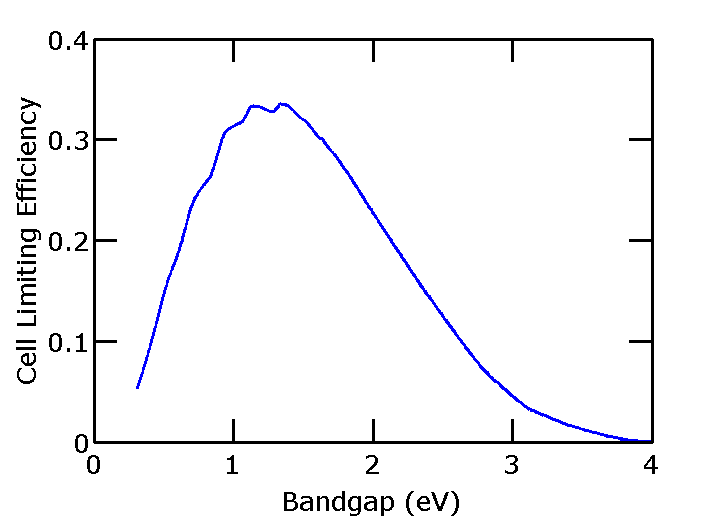
\includegraphics[scale=.4]{Figures/LimitingEfficiencyVersusEnergy2}
 \caption{Limiting Efficiency versus Band gap energy}
  \label{fig:LimitingEfficiency}
\end{figure}
We get a maximum of 33.12\% at a bandgap of 1.34 eV.  
This is very close to the 33.16\% and bandgap of 1.34 eV in this reference \cite{Ruhle:16}.

%\subsubsection{Slight Accuracy Improvement}
%
%In the dark, 
%\begin{equation}
%J = J_{th} - J_{rad}
%\end{equation}
%\begin{equation}
%J_{rad} = q \int_{E_g}^{\infty}  b_e (E, \Delta \mu)  dE
%\end{equation}
%\begin{equation} 
%J_{th} = q \int_{E_g}^{\infty} b_e (E, 0) dE
%\end{equation}
%In the light, 
%\begin{equation}
%J = J_s - [J_{rad} -J_{th}] 
%\end{equation}
%\begin{equation}
%J_s = q \int_{E_g}^{\infty} b_s(E) dE
%\end{equation}
%and $J_{rad}$ is the same.  However, $J_{th}$ is now, 
%\begin{equation}
%J_{th} = q \int_{E_g}^{\infty} \left ( 1 - \frac{F_s}{F_e}  \right ) b_e (E, 0) dE
%\end{equation}
%since a small fraction of thermal photons has been replaced by solar photons.  
%\begin{equation}
%J = q \int_{E_g}^{\infty} \left [ b_s(E) - \frac{F_s}{F_e} b_e(E, 0) \right ] dE - q \int_{E_g}^{\infty}   \left [ b_e (E, \Delta \mu)  - b_e (E, 0) \right ]  dE 
%\end{equation}

\subsection{Tandem Cells}



Consider $n$ solar cells in tandem \cite{Vos:80}.  The band gaps of the $N$ solar cells are 
$E_{g1}, E_{g2},\ldots E_{gN}$ and arranged $E_{g1} \geq E_{g2} \geq \ldots E_{gN}$.  


The current-voltage characteristic of the $i$th cell is 
\begin{equation}
\begin{aligned}
J_i(V_i) &= J_{0i} \left [ \exp (q V_i/k T) - 1 \right ] - J_{1i}
\end{aligned}
\end{equation}
The reverse saturation current $I_{0i}$ is determined by 
\begin{equation}
J_{0i} = q F_{0i} = 2 q \int_{E_{gi}/h}^{\infty} N(\nu, T) d \nu
\end{equation}
\blue{Why is there a factor of two?}
\begin{equation}
N( \nu, T) = \frac{ 2 \pi}{c^2} \frac{\nu^2}{\exp (h \nu/ k T) - 1} 
\end{equation}
Since $E = h \nu$, 
then, 
\begin{equation}
N( E, T) = \frac{ 2 \pi}{h^2 c^2} \frac{E^2}{\exp (E/ k T) - 1}
\end{equation}
and $d \nu = d E/h$.  
Thus, 
\begin{equation}
J_{0i} = q F_{0i} = 2 q \int_{E_{gi}}^{\infty} N(E, T) d E/h = 2 q \int_{E_{gi}}^{\infty} b_e(E) d E
\end{equation}
where 
\begin{equation}
b_e(E) = \frac{ 2 \pi}{h^3 c^2} \frac{E^2}{\exp (E/ k T) - 1}.
\end{equation}
The factor of two comes from emission into all directions as opposed to just plane emitting into air.  

The light-generated current is given by 
\begin{equation}
J_{1i} = q ( F_{si} - F_{0i} )
\end{equation}
\blue{Why is there the second term?  Seems like all of thermal photons replaced by solar photons.
Think this will be similar because $F_{si} >> F_{0i}$, but still not sure why it is included.}

For the top layer, 
\begin{equation}
F_{s1} = \int_{E_{g1}}^{\infty} b_s(E) dE + \int_{E_{g1}}^{\infty} b_e(E) dE \exp (q V_2/ k T)
\end{equation}
The second term is emission from below.  

For cells $i = 2, 3, \ldots, N - 1$
\begin{equation}
F_{si} = \int_{E_{gi}}^{E_{g(i-1)}} b_s(E) dE  + \int_{E_{g(i-1)}}^{\infty} b_e(E) dE \exp (q V_{i-1}/ k T) + \int_{E_{gi}}^{\infty} b_e(E) dE \exp (q V_{i+1}/ k T) 
\end{equation}
The second term is emission from the cell above and the third term is emission from the cell below.

The last solar cell is 
\begin{equation}
F_{sN} = q \int_{E_{gN}}^{E_{g(N-1)}} b_s(E) dE + \int_{E_{g(N-1)}}^{\infty} b_e(E) dE \exp (q V_{N-1}/ k T)
\end{equation}
where the second term is emission from the cell above.  
The total electrical power is 
The total electrical power generated by the system is 

\begin{equation}
P = - \sum_{i = 1}^{N} V_i I_i
\end{equation}

%
%\begin{equation}
%\begin{aligned}
%%I_i(V_i) = I_{0i} \left [ \exp (q V_i/k T) - 1 \right ] - I_{1i}
%J_i(V_i) &= J_{darki} - J_{sci} \\
%&= J_{0i} \left [ \exp (q V_i/ k T) \right ] - J_{sci} %\left [ \exp (q V_i/k T) - 1 \right ] - I_{1i}
%\end{aligned}
%\end{equation}
%where $J_{0i} \left [ \exp (q V_i/ k T) \right ]$ is the dark current.  
%
%The dark current may be determined from 
%\begin{equation}
%J_{darki}(V) = q \int_{0}^{\infty} b_e (E)  dE \exp (q V_i/ k T)
%\end{equation}
%or 
%\begin{equation}
%J_{0i} = q \int_{0}^{\infty} b_e (E)  dE
%\end{equation}
%
%The first cell is illuminated by the sun and the light emitted by the second cell:
%\begin{equation}
%J_{sc1} = q \int_{E_{g1}}^{\infty} b_s(E) dE + \int_{E_{g1}}^{\infty} b_e(E) dE \exp (q V_2/ k T)
%\end{equation}
%
%For cells $i = 2, 3, \ldots, N - 1$
%\begin{equation}
%J_{sci} = q \int_{E_{gi}}^{E_{g(i-1)}} b_s(E) dE + \int_{E_{gi}}^{\infty} b_e(E) dE \exp (q V_{i+1}/ k T)  + \int_{E_{g(i-1)}}^{\infty} b_e(E) dE \exp (q V_{i-1}/ k T)
%\end{equation}
%where the first term is the part of the solar spectrum absorbed, the second term is the light emitted by the cell below and the third term is the light emitted by the cell above.  
%
%The last cell in the stack is only illuminated by the cell above and thus is 
%\begin{equation}
%J_{scN} = q \int_{E_{gN}}^{E_{g(N-1)}} b_s(E) dE + \int_{E_{g(N-1)}}^{\infty} b_e(E) dE \exp (q V_{N-1}/ k T)
%\end{equation}



The maximum power is at $\frac{\partial P}{\partial V_i} = 0$.  

Let $x_i = q V_i/k T$.  
Then the system of equations is 

\begin{equation}
\begin{aligned}
J_1(V_1) &= J_{01} \left [ \exp (q V_1/ k T) - 1 \right ] - J_{11} \\
J_2(V_2) &= J_{02} \left [ \exp (q V_2/ k T) -1  \right ] - J_{12} \\
\vdots \\
J_N(V_N) &= J_{0N} \left [ \exp (q V_N/ k T) -1 \right ] - J_{1N} 
\end{aligned}
\end{equation}
or 
\begin{equation}
\begin{aligned}
J_1(V_1) &= q F_{01} \left [ \exp (q V_1/ k T) - 1 \right ] - q (F_{s1} - F_{01})  \\
J_2(V_2) &= q F_{02} \left [ \exp (q V_2/ k T) -1  \right ] - q (F_{s2} - F_{02})\\
\vdots \\
J_N(V_N) &= q F_{0N} \left [ \exp (q V_N/ k T) -1 \right ] - q (F_{sN} - F_{0N}) 
\end{aligned}
\end{equation}
The $F_{0i}$ terms are independent of $V_i$.  However, the $F_{si}$ terms are dependent on $V_i$.  
\begin{equation}
\begin{aligned}
J_1(V_1) &= q F_{01} \left [ \exp (q V_1/ k T) - 1 \right ] - q \left ( \left [ \int_{E_{g1}}^{\infty} b_s(E) dE + \int_{E_{g1}}^{\infty} b_e(E) dE \exp (q V_2/ k T) \right ] - F_{01} \right )  \\
J_2(V_2) &= q F_{02} \left [ \exp (q V_2/ k T) -1  \right ] \ldots \\
& - q \left ( \left [ \int_{E_{g2}}^{E_{g1}} b_s(E) dE  + \int_{E_{g1}}^{\infty} b_e(E) dE \exp (q V_{1}/ k T) + \int_{E_{g2}}^{\infty} b_e(E) dE \exp (q V_{3}/ k T)  \right ] - F_{02} \right )\\
J_i(V_i) &= q F_{0i} \left [ \exp (q V_i/ k T) -1  \right ] \ldots \\
& - q \left ( \left [ \int_{E_{gi}}^{E_{g(i-1)}} b_s(E) dE  + \int_{E_{g(i-1)}}^{\infty} b_e(E) dE \exp (q V_{i-1}/ k T) + \int_{E_{gi}}^{\infty} b_e(E) dE \exp (q V_{i+1}/ k T)  \right ] - F_{0i} \right )\\
\vdots \\
J_N(V_N) &= q F_{0N} \left [ \exp (q V_N/ k T) -1 \right ] \ldots \\
&- q \left ( \left [  \int_{E_{gN}}^{E_{g(N-1)}} b_s(E) dE + \int_{E_{g(N-1)}}^{\infty} b_e(E) dE \exp (q V_{N-1}/ k T)   \right ] - F_{0N} \right ) 
\end{aligned}
\end{equation}
\begin{equation}
\begin{aligned}
\frac{\partial P}{\partial V_1} &= 0 \\
&= J_1 + \frac{\partial J_1}{\partial V_1} V_1 + \frac{\partial J_2}{\partial V_1} V_2 \\
&= \left \{ q F_{01} \left [ \exp (q V_1/ k T) - 1 \right ] - q (F_{s1} - F_{01}) \right \} + \left \{ q F_{01} \exp (q V_1/ k T) \frac{q}{k T} V_1 \right \} \ldots \\
& -q \left \{ \int_{E_{g1}}^{\infty} b_e(E) dE \exp (q V_{1}/ k T) \frac{q}{k T} V_2  \right \}
\end{aligned}
\end{equation}
Rearranging, we get
\begin{equation}
\begin{aligned}
F_{01} \exp (\frac{ q V_1}{ k T} ) \left ( 1 + \frac{ q V_1}{k T} \right ) & = F_{s1} + \int_{E_{g1}}^{\infty} b_e(E) dE \exp (q V_{1}/ k T) \frac{q}{k T} V_2 \\
F_{01} \exp x_1 (1 + x_1) &= F_{s1} + \frac{1}{2} F_{01} x_2 \exp x_1 \\
\exp x_1 (1 + x_1) &= \frac{F_{s1}}{F_{01}} + \frac{1}{2} x_2 \exp x_1 
\end{aligned}
\end{equation}
because $\frac{1}{2} F_{01} = \int_{E_{g1}}^{\infty} b_e(E) dE$

For the second equation, 
\begin{equation}
\begin{aligned}
\frac{\partial P}{\partial V_2} &= 0 \\
&= J_2 + \frac{\partial J_1}{\partial V_2} V_1 + \frac{\partial J_2}{\partial V_2} V_2 + \frac{\partial J_3}{\partial V_2} V_3 \\
&= q F_{02} \left [ \exp (q V_2/ k T) - 1 \right ] - q (F_{s2} - F_{02})  \ldots \\
&- q \int_{E_{g1}}^{\infty} b_e(E) dE \exp (q V_2/ k T) \frac{q}{k T} V_1 \ldots \\
&+  q F_{02} \exp (q V_2/ k T) \frac{q}{k T} V_2  \ldots \\
& -q  \int_{E_{g2}}^{\infty} b_e(E) dE \exp (q V_{2}/ k T) \frac{q}{k T} V_3  
\end{aligned}
\end{equation}
Rearranging, we get
\begin{equation}
\begin{aligned}
F_{02} \exp (\frac{ q V_2}{ k T} ) \left ( 1 + \frac{ q V_2}{k T} \right ) & = F_{s2} + 
\int_{E_{g1}}^{\infty} b_e(E) dE \exp (q V_2/ k T) \frac{q}{k T} V_1 + 
\int_{E_{g2}}^{\infty} b_e(E) dE \exp (q V_{2}/ k T) \frac{q}{k T} V_3 \\
F_{02} \exp x_2 \left ( 1 + x_2 \right ) & = F_{s2} + 
\int_{E_{g1}}^{\infty} b_e(E) dE \exp (x_2) x_1 + 
\frac{1}{2} F_{02} \exp (x_2) x_3  \\
\left ( 1 + x_2 \right )  \exp x_2  & = \frac{F_{s2}}{F_{02}} + 
x_1 \exp (x_2)  \frac{\int_{E_{g1}}^{\infty} b_e(E) dE}{F_{02}}   + 
\frac{1}{2} x_3 \exp (x_2)   \\
\left ( 1 + x_2 \right )  \exp x_2  & = \frac{F_{s2}}{F_{02}} + 
\frac{1}{2} x_1 \exp (x_2)  \frac{\int_{E_{g1}}^{\infty} b_e(E) dE}{\int_{E_{g2}}^{\infty} b_e(E) dE}   + 
\frac{1}{2} x_3 \exp (x_2)  
\end{aligned}
\end{equation}
In general, 
\begin{equation}
\left ( 1 + x_i \right )  \exp x_i   = \frac{F_{si}}{F_{0i}} + 
\frac{1}{2} x_{i-1} \exp (x_i)  \frac{\int_{E_{g(i-1)}}^{\infty} b_e(E) dE}{\int_{E_{gi}}^{\infty} b_e(E) dE}   + 
\frac{1}{2} x_{i+1} \exp (x_i)  
\end{equation}

For the $N$th equation, 
\begin{equation}
\begin{aligned}
\frac{\partial P}{\partial V_N} &= 0 \\
&= J_N + \frac{\partial J_{N-1}}{\partial V_N} V_{N-1} + \frac{\partial J_N}{\partial V_N} V_N \\
&= q F_{0N} \left [ \exp (q V_N/ k T) - 1 \right ] - q (F_{sN} - F_{0N})  \ldots \\
&- q \int_{E_{g(N-1)}}^{\infty} b_e(E) dE \exp (q V_N/ k T) \frac{q}{k T} V_{N-1} \ldots \\
&+  q F_{0N} \exp (q V_N/ k T) \frac{q}{k T} V_N   
\end{aligned}
\end{equation}
Rearranging, we get
\begin{equation}
\begin{aligned}
F_{0N} \exp (\frac{ q V_N}{ k T} ) \left ( 1 + \frac{ q V_N}{k T} \right ) & = F_{sN} + 
\int_{E_{g(N-1)}}^{\infty} b_e(E) dE \exp (q V_N/ k T) \frac{q}{k T} V_{N-1} \\
F_{0N} \exp x_N \left ( 1 + x_N \right ) & = F_{sN} + 
\int_{E_{g(N-1)}}^{\infty} b_e(E) dE \exp (x_N) x_{N-1} \\
 \exp x_N \left ( 1 + x_N \right ) & = \frac{F_{sN}}{F_{0N}} + 
\exp (x_N) x_{N-1} \frac{\int_{E_{g(N-1)}}^{\infty} b_e(E) dE}{F_{0N}}  \\
\left ( 1 + x_N \right ) \exp x_N  & = \frac{F_{sN}}{F_{0N}} + 
x_{N-1} \frac{1}{2} \exp (x_N)  \frac{\int_{E_{g(N-1)}}^{\infty} b_e(E) dE}{\int_{E_{gN}}^{\infty} b_e(E) dE}  \\
\end{aligned}
\end{equation}

The system of equations is thus, 
\begin{equation}
\begin{aligned}
(1 + x_1) \exp x_1  &= \frac{F_{s1}}{F_{01}} + \frac{1}{2} x_2 \exp x_1 \\
\left ( 1 + x_i \right )  \exp x_i   &= \frac{F_{si}}{F_{0i}} + 
\frac{1}{2} x_{i-1} \exp (x_i)  \frac{\int_{E_{g(i-1)}}^{\infty} b_e(E) dE}{\int_{E_{gi}}^{\infty} b_e(E) dE}   + 
\frac{1}{2} x_{i+1} \exp (x_i)   \\
\left ( 1 + x_N \right ) \exp x_N  & = \frac{F_{sN}}{F_{0N}} + 
\frac{1}{2} x_{N-1}  \exp (x_N)  \frac{\int_{E_{g(N-1)}}^{\infty} b_e(E) dE}{\int_{E_{gN}}^{\infty} b_e(E) dE}  \\
\end{aligned}
\end{equation}

Let us designate 
\begin{equation}
F_{0ti} = \int_{E_{gi}}^{\infty} b_e(E) dE.
\end{equation}
This term appears in $F_{0i}$ and the gradient.  

%Numerical approach, 
%\begin{enumerate}
%\item Calculate $F_{0i}$.  These are independent of $V_{i}$.  Calculate various $\int_{E_{gi}}^{\infty} b_e(E) dE$ terms.  
%Each $F_{si}$ is a function of $V_{i-1}$, $V_{i}$, and $V_{i+1}$.  
%\item Use Newton's method,
%\begin{enumerate}
%\item Guess a set of $\mathbf{V_0}$.  
%\item Obtain the value of system of equations which is supposed to equal 0, $\mathbf{f} (\mathbf{V_0})$.
%\item Get matrix of partial derivatives, $D \mathbf{f} (\mathbf{V_0})$
%\item Solve the equation $D \mathbf{f} (\mathbf{V_0}) \Delta \mathbf{V} = - \mathbf{f} (\mathbf{V_0})$
%\item Get next iteration, $\mathbf{V_1} =\mathbf{V_0} + \Delta \mathbf{V}$
%\item Continue steps (c) through (e).  Step when matrix of partial derivatives is small.  
%\end{enumerate}
%
%\item Use \textbf{steepest descent} method,
%\begin{enumerate}
%\item Guess a set of $V_{i}$, $\mathbf{V_0}$.  
%%\item Obtain the power, $P$.
%\item Get gradient, $\nabla P (\mathbf{V_0})$, which is simply vector of partial derivatives, $\left ( \frac{\partial P}{\partial V_1},  \frac{\partial P}{\partial V_2}, \ldots \frac{\partial P}{\partial V_N} \right )$
%\item Move from point $\mathbf{V_i}$ to the point $\mathbf{V_{i+1}}$ by minimizing along the line from $\mathbf{V_i}$ in the direction of the 
%local downhill gradient $- \nabla P (\mathbf{V_i})$.  
%%, $\mathbf{V_1} =\mathbf{V_0} + \Delta \mathbf{V}$
%\end{enumerate}
%The method will perform many small steps in going down a long, narrow valley, even if the valley is a
%perfect quadratic form.  It is better to proceed in a direction that is conjugate to all previous directions traveled.  
%
%%\item Use \textbf{direction set method} due to Powell.  This requires a one-dimensional minimization (such as Brent's method)   
%%\begin{enumerate}
%%\item 
%%\end{enumerate}
%
%\item Use \textbf{conjugate gradient method}, such as the Polak Ribiere method.  This requires $N$ storage, derivative calculations, and one-dimensional sub minimization.  
%\begin{enumerate}
%\item Set $\mathbf{g}_0 = - \nabla f (\mathbf{V}_0)$ for some initial guess $\mathbf{V}_0$.  Let $\mathbf{h_0} = \mathbf{g_0}$
%\item Move along the direction $\mathbf{h_0}$ to the local minimum of $P$ located at some point $\mathbf{V_{1}}$.
%\item Set $\mathbf{g}_{1} = - \nabla f (\mathbf{V}_{1})$
%%\item Start with an arbitrary initial vector $\mathbf{g_0}$.  Let $\mathbf{h_0} = \mathbf{g_0}$.  
%\item $\gamma_0 = \frac{\mathbf{g}_{1} \cdot \mathbf{g}_{1}}{\mathbf{g}_0 \cdot \mathbf{g}_0}$ for Fletcher Reeves,\\
%or $\gamma_0 = \frac{( \mathbf{g}_{1}- \mathbf{g}_0 ) \cdot \mathbf{g}_{1}}{\mathbf{g}_0 \cdot \mathbf{g}_0}$ for Polak-Ribiere\\
%$\mathbf{h_{1}} = \mathbf{g}_{1} + \gamma_0 \mathbf{h}_0$. 
%\item 
%Get $\mathbf{g_{i+1}}$ by moving along the direction $\mathbf{h_i}$ to the local minimum of $f$ located at some point $\mathbf{P_{i+1}}$. Set $\mathbf{g_{i+1}} = - \nabla f (\mathbf{P_{i+1}})$ % $\mathbf{g_{i+1}} = \mathbf{g_i} - \lambda_i \mathbf{A} \cdot \mathbf{h_i}$ 
%
%\item $\gamma_i = \frac{\mathbf{g_{i+1}} \cdot \mathbf{g_{i+1}}}{\mathbf{g_i} \cdot \mathbf{g_i}}$ for Fletcher Reeves,\\
% or for Polak-Ribiere, $\gamma_i = \frac{( \mathbf{g}_{i+1}- \mathbf{g}_i ) \cdot \mathbf{g}_{i+1}}{\mathbf{g}_i \cdot \mathbf{g}_i}$ \\
%$\mathbf{h_{i+1}} = \mathbf{g_{i+1}} + \gamma_i \mathbf{h_i}$. 
%%Set $\mathbf{g}_i = - \nabla f (\mathbf{P}_i)$ for some point $\mathbf{P}_i$.
%\end{enumerate}
%\end{enumerate}
%Pseudocode for this
%\begin{enumerate}
%\item Set maximum number of iterations, epsilon for convergence of solution, and gradient tolerance
%\item $n$ is size of vector $p$
%\item $p$ = $pp$ \blue{why?}
%
%\end{enumerate}

Use Matlab, \texttt{fminunc} with gradient information.

%For one-dimensional optimization, can use Brent's method:
%\begin{enumerate}
%\item 
%\end{enumerate}


\section{Absolute Limiting Efficiency}



\subsection{Geometrical Factors}
The energy current emitted from a sphere (the sun) with radius $R_s$ to the earth is exactly the same as that of a flat disc with radius $R_s$ oriented perpendicularly to the line connecting to the line connecting the earth and the sun.  See \cite{Wurfel:09} Section 2.1.3.

In spherical coordinates, the solid angle is 
\begin{equation}
\boxed{d \Omega = \sin \theta d \theta d \psi.}
\end{equation}

For a cone with apex angle $2 \theta$, the solid angle is 

\begin{equation}
\Omega = 2 \pi \int_0^{\theta} \sin \theta d \theta = 2 \pi (1 - \cos \theta) = 4 \pi \sin^2 (\frac{\theta}{2}).
\end{equation}
The sun subtends an angle $\theta_s = 16' = 0.26^{\circ}$. Thus, 
\begin{equation}
\boxed{\Omega_s = 2.1662 \times 10^{-5} \pi = 6.8052 \times 10^{-5}}
\end{equation}

For small $\theta$, $\Omega = 2 \pi \sin^2\theta$.  
For a spherical cap, $\theta = \pi$ and thus, $\Omega = 4 \pi$, and for a hemispherical cap $\theta = \pi/2$ and thus, $\Omega = 2 \pi$.  

For a surface element, $\Omega = \pi$.  





%From the earth, 
\subsection{Restriction of Solid Angle}
%$\theta_s$ 
The sun radiation reaches the cell within solid angle $2 \theta_X$, which can be equal to that subtended by the sun or greater due to the use of optical concentrators.  

For optical concentrators, 
\begin{equation}
X \sin^2{\theta_s} = \sin^2{\theta_X}
\end{equation}
where $X$ is the concentration ratio. 
Photons are emitted through solid angle $2 \theta_E$, where $\theta_E \geq \theta_X$.  $\theta_E = \pi/2$ typically.
%in a typical solar cell.  


We define
%\begin{equation}
%b (E, T) = \frac{2}{h^3 c^2} \frac{E^2}{\exp(E/kT) - 1},
%\end{equation}
\begin{equation}
b (E, T, V) = \frac{2}{h^3 c^2} \frac{E^2}{\exp\left [(E-qV)/kT \right ] - 1}, 
\end{equation}
and
\begin{equation}
\Gamma_X = \pi \sin^2 \theta_X, \\
\Gamma_E = \pi \sin^2 \theta_E,
\Gamma_s = \pi \sin^2 \theta_s,
\end{equation}
where the factor of 2 has been removed for a flat plate emitting into some angle.  $\theta_s = 0.26^{\circ}$ for the sun.  

The absolute limiting efficiency is calculated in \cite{Araujo:94}.  
The current is
\begin{equation}
J(V) = q \int_{E_g}^{\infty} \left \{ \Gamma_X \left [ b (E, T_s,0) - b(E, T_c, 0) \right ] - \Gamma_E  \left [ b(E, T_c, V)  - b(E, T_c, 0) \right ]  \right \}  dE
\end{equation}

In \textbf{solar concentration}, we increase $\Gamma_X$.   The highest concentration possible is when $X = 1/\sin^{2} \theta_s$, $\theta_x = \pi/2$, and $\Gamma_X = \pi$.   

In \textbf{emission angle restriction}, we decrease $\Gamma_E$.   We restrict $\theta_E = \theta_X = \theta_s$ to obtain maximum efficiency.  It should be noted, the conversion efficiency does not depend on concentration.     
%The highest concentration possible is when $X = 1/\sin^{2} \theta_s$, $\theta_x = \pi/2$, and $\Gamma_X = \pi$.   


Using the photon flux density of the AM1.5 solar spectrum, the current is
\begin{equation}
J(V) = q \int_{E_g}^{\infty} \left \{ \Gamma_X \left [ \frac{b_s}{\Gamma_s} -  b(E, T_c, 0) \right ] - \Gamma_E  \left [ b(E, T_c, V)  - b(E, T_c, 0) \right ]  \right \}  dE.
\end{equation}

%\begin{equation}
%J(V) = q  \int_{E_g}^{\infty} \left \{ b_s (E) - \sin^{2} \theta_E  \left [ b_e(E, V)  - b_e(E,0) \right ]  - 
%\frac{\sin^2 \theta_x}{\Omega_a} b_e(E,0)  \right \}  dE
%\end{equation}
%$\Omega_a = \pi$, which is the geometrical factor for a thin film radiating into a hemisphere.  
In the limit, with $\theta_E = \frac{\pi}{2}$, $\Gamma_E = \pi$.   
and $\Gamma_X b(E, T_c, 0) \approx 0$, we recover the limiting efficiency.    

\subsection{Non-Idealities}


\subsubsection{Internal Fluorescence}

In the case of internal fluoresce yield $\eta_{int}$, the current is
\begin{equation}
J(V) = q \int_{E_g}^{\infty} \left \{ \Gamma_X \left [ b (E, T_s,0) - b(E, T_c, 0) \right ] - \Gamma_E  \left [ b(E, T_c, V)  - b(E, T_c, 0) \right ]  \right \} A(E) dE
\end{equation}



%where $F_s$ is a 


\section{Angle Dependent Properties}

When the incidence angle is off from normal, the short-circuit current density is 
\begin{equation}
J_{sc} = q \int_{0}^{\infty} b_s(E) A(E) dE \cos \theta.
\end{equation}
where $\theta$ is the angle from the normal.  
This is because the photon flux density has decreased by $\cos \theta$.

Similarly, the ultimate efficiency is 
\begin{equation}
\begin{aligned}
\eta_{ue} &= \frac{\int_{E_g}^{\infty} I(E) A(E) \frac{E_g}{E} dE}{\int_{0}^{\infty} I(E) dE} \cos \theta\\
&= \frac{ E_g  \int_{E_g}^{\infty} b_s(E) A(E) dE \cos \theta}{\int_{0}^{\infty} I(E) dE} 
\end{aligned}
\end{equation}
for the same reasons as above.  Note, the open circuit voltage is $E_g/q$ and the short-circuit current density is the same as above.  

\subsection{Maximum Absorption Enhancement}
The maximum absorption enhancement is 
\begin{equation}
f_{max} = 4 n^2/ \sin^2(\theta_c)
\end{equation}
where $\theta$ is half of the apex angle of the absorption cone.  
For the isotropic case where $\theta_c = 90^{\circ}$, $f_{max} = 4 n^2$ \cite{Yablonovitch:82july}.  

For general light trapping case \cite{Yu:11},
\begin{equation}
F = \int_0^{\pi/2} \int_{0}^{2 \pi} f(\theta, \phi) \cos \theta \sin \theta d \theta d \phi \leq 4 \pi n^2
\end{equation}
This is applicable for a film that is internally uniform and has a thickness of a few wavelengths.  
Using density of states, 
\begin{equation}
\sum_n f_n \leq \frac{2 \pi c}{n d} \rho (\omega)
\end{equation}


%The absorption is
%\begin{equation}
%A_{\Omega} = \int_0^{2 \pi}\int^{\frac{\pi}{2}}_0 A_{solar}(\theta, \phi) \cos \theta \sin \theta d\theta d\phi . \label{eq:angleIntegrated}
%\end{equation}
%
%
%
%
%In spherical coordinates, the solid angle is 
%\begin{equation}
%d \Omega = \sin \theta d \phi d \theta 
%\end{equation}
%
%$A_{solar}(\theta, \phi)$ is still from 0 to 1.  
%Assuming, $A_{solar}(\theta, \phi) = 1$ everywhere, you get $A_{\Omega} = \pi$.  
%$A_{solar}(\theta, \phi)$ must also be averaged over the two polarizations.  



\section{Absorption per Unit Volume}

The electric field intensity is 
\begin{equation}
| \mathbf{E}(\mathbf{r, E}) |^2 = | \tilde{\mathbf{E}}(\mathbf{r}, E) |^2 \frac{I(E) Area }{P_{in}(E)}.
\end{equation}
where $| \tilde{\mathbf{E}}(\mathbf{r}, E) |^2$ is the electric field intensity of the simulation, $Area$ is the area of the simulation, and $P_{in}$ is the power of the simulation.


The weighted electric field intensity is 
\begin{equation}
| \mathbf{E}(\mathbf{r}) |^2 = \int_0^{\infty}  | \mathbf{E}(\mathbf{r}, E) |^2 \frac{I(E) Area~dE}{P_{in}(E)}.
\end{equation}


The position dependent absorption per unit volume may be calculated from the divergence of the Poynting vector $\vec{P}$:
\begin{equation} 
\tilde{A}(\mathbf{r}, E) = \frac{1}{2} \mathrm{real} \{ {\vec{\nabla} \cdot \vec{P}} \} = \frac{1}{2} \epsilon_i(E) \frac{E}{\hbar}  \left| \tilde{\mathbf{E}}(\mathbf{r}, E) \right|^2
\end{equation}
in units of (W/m$^3$).  The absorption $A(\mathbf{r}, E)$ in units of 1/m$^3$ may be obtained be normalizing $\tilde{A}(\mathbf{r}, E)$ over the incoming radiation power, 
$A(\mathbf{r}, E) = \frac{\tilde{A}(\mathbf{r}, E)}{P_{in}}$.  Integrating over the volume gives us $A(E)$ from 0 to 1: $A(E) = \int A(\mathbf{r}, E) dV$.  

The spectrally weighted absorption is
\begin{align} 
\bar{A}(\mathbf{r}, E) &= \frac{1}{2} \mathrm{real} \{ {\vec{\nabla} \cdot \vec{P}} \} = \frac{1}{2} \epsilon_i(E) \frac{E}{\hbar}  \left| \tilde{\mathbf{E}}(\mathbf{r}, E) \right|^2 \frac{I(E) Area}{P_{in}} \\
&= A(\mathbf{r}, E) I(E) Area \\
&= \tilde{A}(\mathbf{r}, E) \frac{I(E) Area}{P_{in}}
\end{align}
in units of W/m$^3$.

Assuming the absorption of each photon results in one electron-hole pair, the generation rate is calculated from  
\begin{equation}
\tilde{G}(\mathbf{r}, E) = \frac{1}{2 E} \mathrm{real} \{ {\vec{\nabla} \cdot \vec{P}} \} 
= \frac{\epsilon_i(E) \left| \mathbf{E}(\mathbf{r}, E) \right|^2}{2 \hbar}.
\end{equation}
in units of 1/(m$^3$sec).
It should be noted that $\tilde{G}(\mathbf{r}, E) = \frac{\tilde{A}(\mathbf{r}, E)}{E}$.  

The position-dependent generation is 
\begin{equation}
G(\mathbf{r}) = \int_{0}^{\infty} \frac{I(E) Area~\tilde{G}(\mathbf{r}, E)}{P_{in}(E) } dE = \int_{0}^{\infty}  \frac{b_s(E) Area~\tilde{A}(\mathbf{r}, E)}{P_{in}(E)} dE
\end{equation}
in units of 1/(m$^3$sec).  This is often converted to 1/(cm$^3$sec)
\begin{equation}
G(\mathbf{r})dE = \frac{ I(E) Area~\tilde{G}(\mathbf{r}, E)}{P_{in}(E) dE}.
\end{equation}




\section{Absorption of Uniform Plane Wave in Infinite Media}

The index of refraction is $n = n_r - j n_i$, where $n_i > 0$ corresponds to loss.  
For non-magnetic media, the absorption coefficient is defined as 
\begin{equation}
\alpha \equiv \frac{1}{I} \frac{d}{dz} I.
\end{equation}

\begin{equation}
\boxed{\alpha = \frac {2 \omega | n_i |}{c} = \frac{4 \pi}{\lambda}  | n_i | }.
\end{equation}

The time-averaged power flux varies from cross-section to cross-section as $\exp(-\alpha z)$.  
\begin{equation}
I(z) = | \textbf{E} | ^2 = I(0) \exp(-\alpha z)
\end{equation}
where $I(0)$ is the intensity of the electromagnetic radiation at $z = 0$.  

The absorption length is 
\begin{equation}
\boxed{L_\alpha \equiv \frac{1}{\alpha}}.
\end{equation}

\begin{figure}[H]
\centering
\vspace{-10pt}
 \subfloat[]{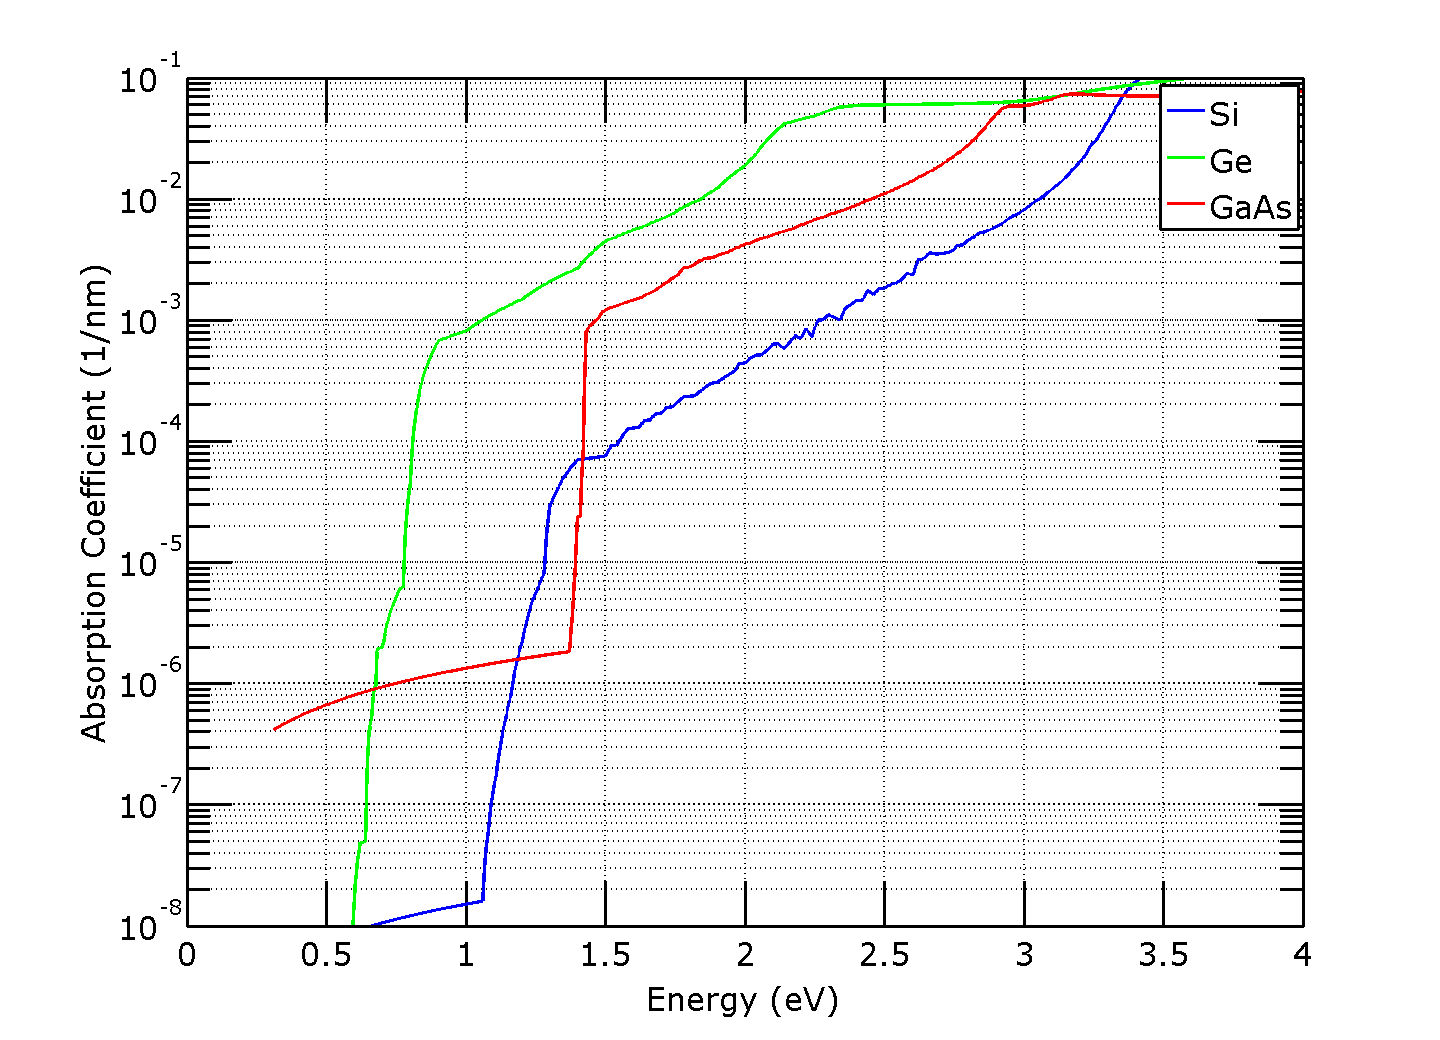
\includegraphics[width=0.45\textwidth]{Figures/AbsorptionCoeffVersusEnergy}}
 \hspace{5pt}
 \subfloat[]{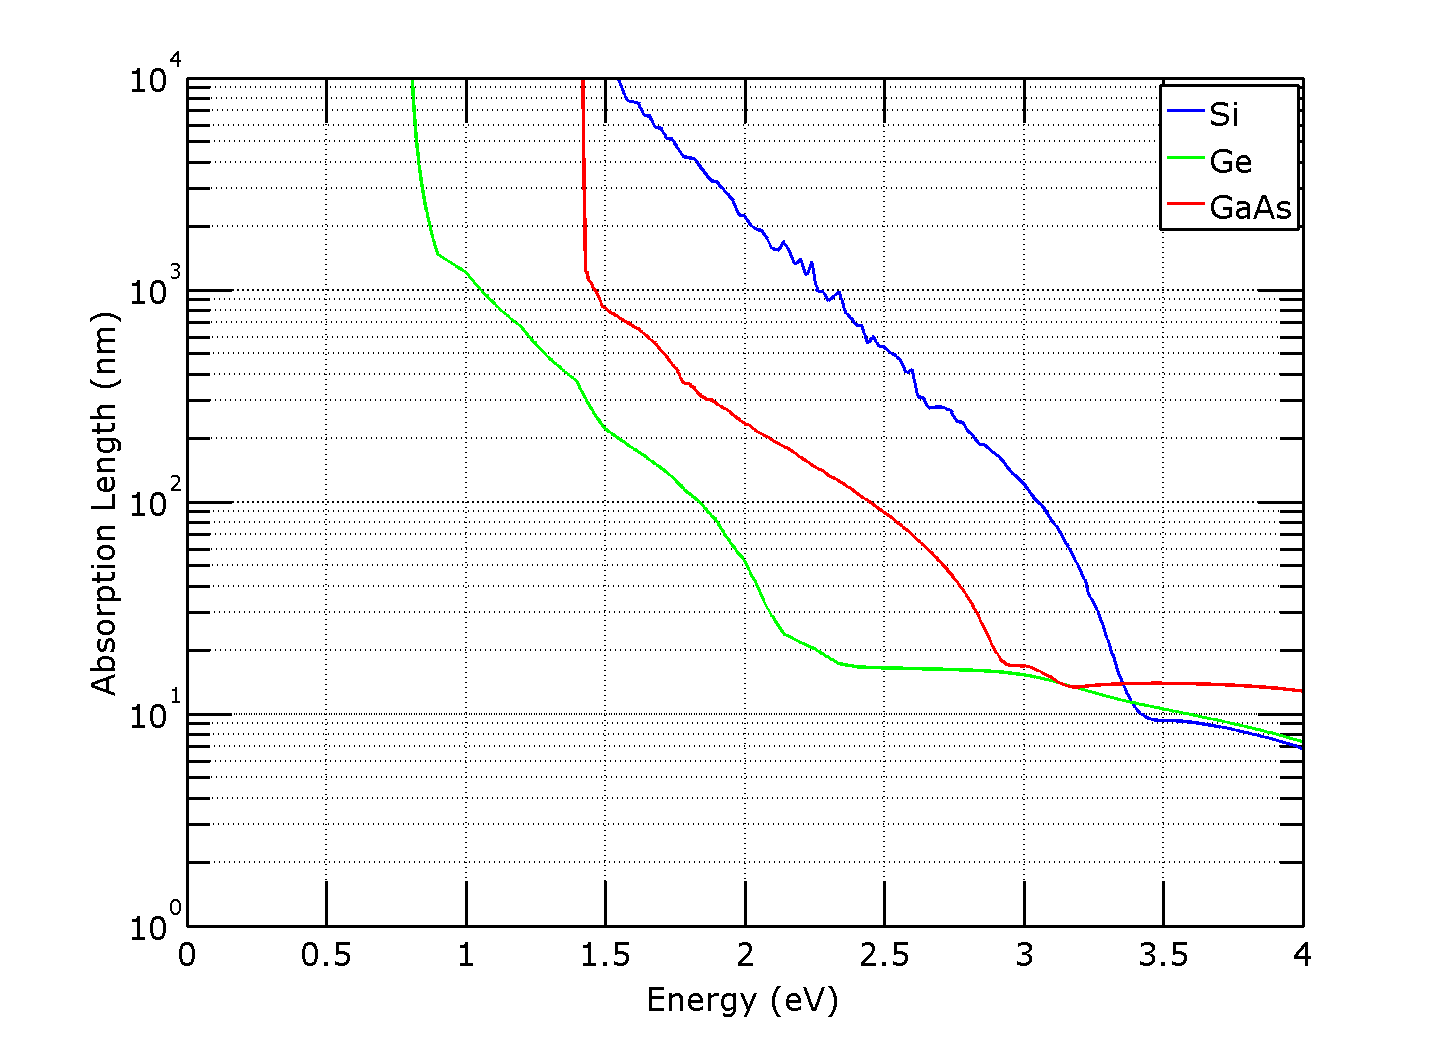
\includegraphics[width=0.45\textwidth]{Figures/AbsorptionLengthVersusEnergy}} 
 \caption[Absorption Coefficient and Absorption Length versus Energy]{Optical Properties of Semiconductors}
  \label{fig:leadingThermoelectrics}
\end{figure}

For a thin film of thickness $L$, assuming that the front surface is perfectly anti reflecting and the back surface is perfectly reflecting, the absorption may be calculated to be $A = 1 - \exp(-2 \alpha L)$, where $\alpha$ is the absorption coefficient of $A$ and $\alpha$ are both functions of $E$.  Here, we use the file ``Si Agrawal extrap.txt" for the optical properties, which is slightly modified with a band gap of about 1.0 eV.  
%The absorption coefficient may be utilized for a thin film of thickness $L$, such that the absorption is equal to .  
\begin{figure}[H]
\centering
\vspace{-10pt}
{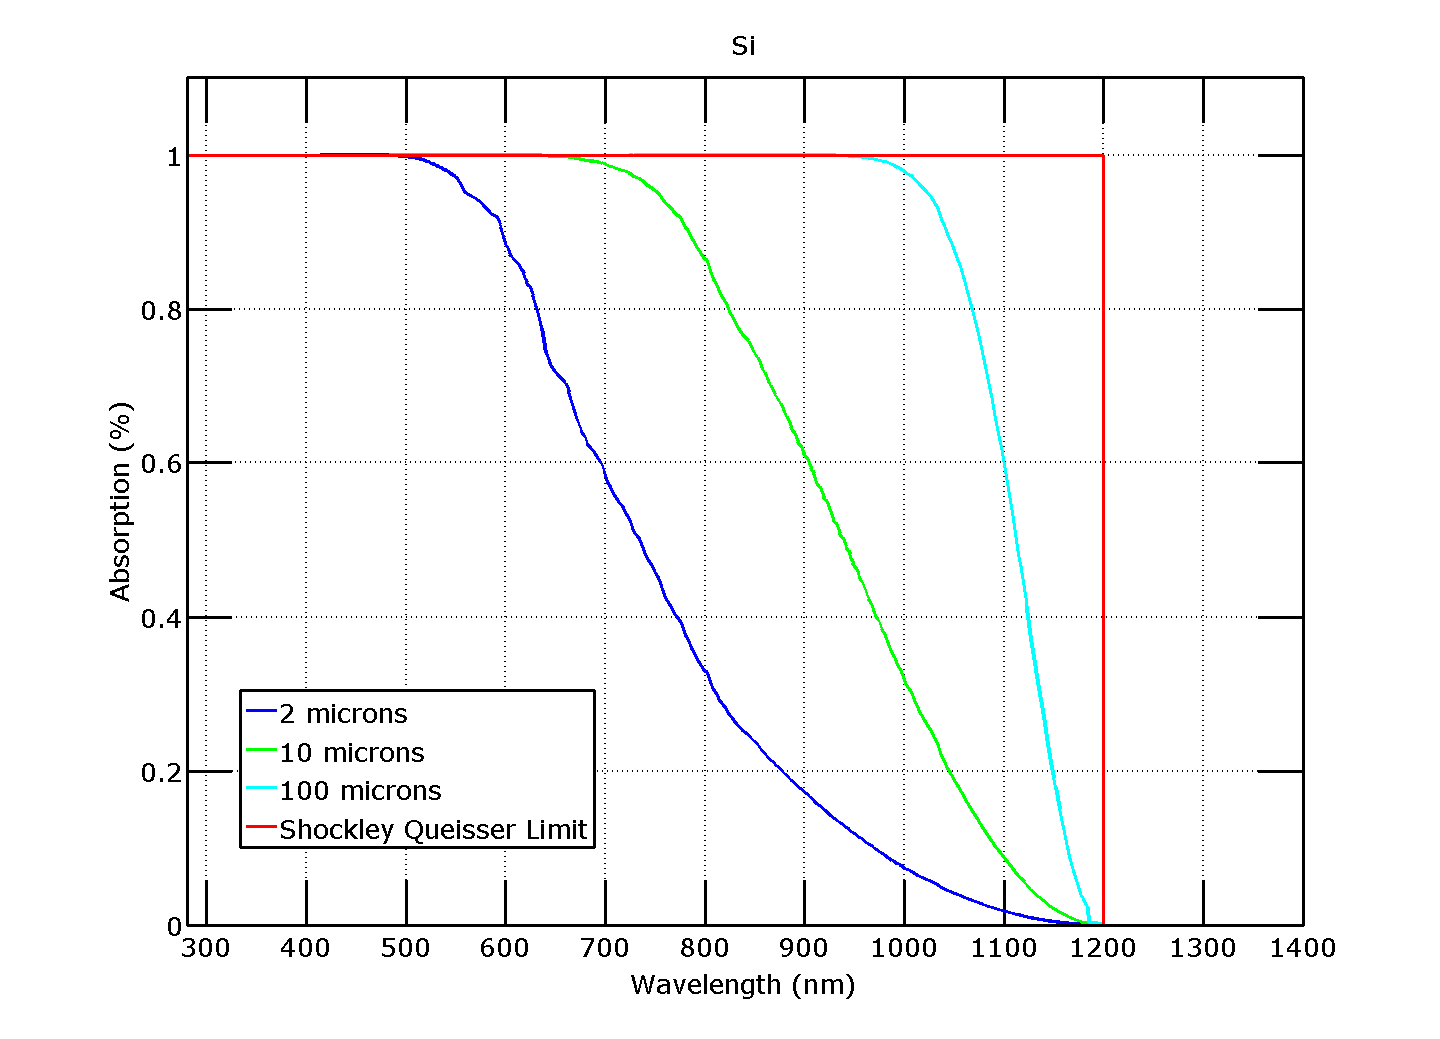
\includegraphics[width=0.45\textwidth]{Figures/SiliconFilmAbsorptionVersusWavelength}} 
 \caption[Silicon absorption for different thickness films]{Silicon absorption for different thickness films.  This assumes perfectly anti-reflecting front surface and perfectly reflecting back surface.}
  \label{fig:absorptionVersusWavelength}
\end{figure}

The limiting efficiency versus thickness may be calculated.  
\begin{figure}[H]
\centering
\vspace{-10pt}
{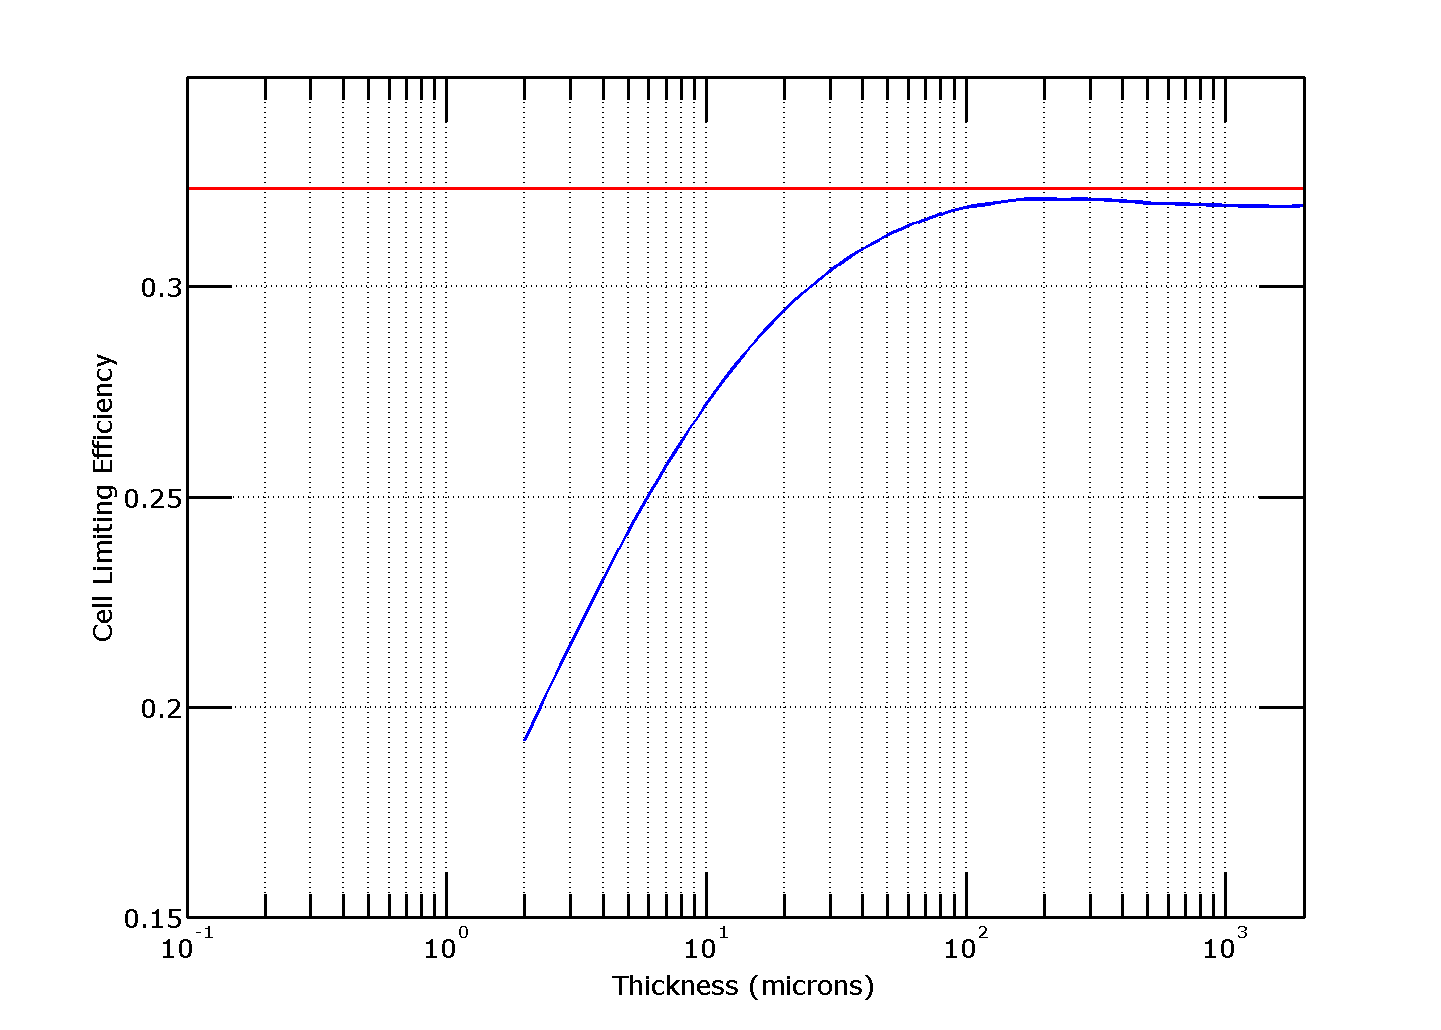
\includegraphics[width=0.45\textwidth]{Figures/LimitingEfficiencyVersusThickness}} 
 \caption[Limiting efficiency considering radiative recombination]{Limiting efficiency considering radiative recombination only versus thickness for silicon.}
  \label{fig:limitingEfficiencyVersusThickness}
\end{figure}

In order to calculate a more detailed limiting efficiency, Auger recombination and free carrier absorption may be considered in addition to radiative recombination \cite{Tiedje:84}.    

The current is now 
\begin{equation}
0 = J_s + J_{th} - J_{rad} - J_{Aug} - J_{fc} - J
\end{equation}
where $J_s$ is the current from solar generation, $J_{th}$ is generation from ambient temperature, $J_{rad}$ is from radiative recombination, $J_{Aug}$ is the Auger recombination current, $J_{fc}$ is the free carrier absorption current, and $J$ is from the extraction of electrons and holes.  

The equation may be reorganized as 
\begin{equation}
J = J_s - [J_{rad} + J_{Aug} + J_{fc} - J_{th}]
\end{equation}
where the term in brackets is the dark current.  

The Auger current is 
\begin{equation}
J_{Aug} = q (C_n n^2 p + C_p p^2 n) V/A.
\end{equation}
where $C_n$ and $C_p$ are Auger coefficients, $V$ is the volume of the material, and $A$ is the area.  
$C = C_n + C_p$ and we assume that the silicon is intrinsic or lightly doped such that $n = p$ under illumination.  
For a thin film, $V/A = L$ where $L$ is the thickness.  Thus, 
\begin{equation}
J_{Aug} = q C n^3 L.
\end{equation}
The carrier concentration may be determined from 
\begin{equation}
n p = n_i p_i \exp\left [ \frac{\mu}{k T} \right ]
\end{equation}
and thus, 
\begin{equation}
\boxed{J_{Aug} = q C n_i^{3} \exp \left [\frac{3 \mu}{2 k T} \right ] L.}
\end{equation}
For silicon, $C = 3.88 \times 10^{-31}$ cm$^{6}$ sec$^{-1}$ and $n_i = 1.45 \times 10^{10}$ cm$^{-3}$.    

\begin{equation}
J_{fc} = \alpha_{fc} q \left ( \int \int A(E) b_n(E, T) dE d\Omega \right) V/A.
\end{equation}
where $\alpha_{fc}$ is the free carrier absorption coefficient, $A(E)$ is the absorption, and $b_n(E, T)$ is the flux of black-body photons for a photon energy interval $dE$ and solid angle $d \Omega$.  For a thin film, $V/A = L$.
\begin{equation}
\boxed{b_{n \Omega} (E, T) = \frac{2 n^2}{h^3 c^2} \frac{E^2}{\exp(E - \Delta \mu)/k T - 1} dE d \Omega}
\end{equation}
For an internal blackbody, the light is radiated from all angles, and thus
\begin{equation}
b_{n} (E, T) = 4 \pi \frac{2 n^2}{h^3 c^2} \frac{E^2}{\exp(E - \Delta \mu)/k T - 1} dE
\end{equation}
Thus, 
\begin{equation}
\boxed{J_{fc} = \alpha_{fc} 4 \pi q L \int A(E) b_n(E, T) dE .}
\end{equation}

By including both Auger recombination and free carrier absorption, the optimum solar cell efficiency is about 29.8 \% at a thickness of $L = 200$ \hbox{\textmu}m
\begin{figure}[H]
\centering
\vspace{-10pt}
{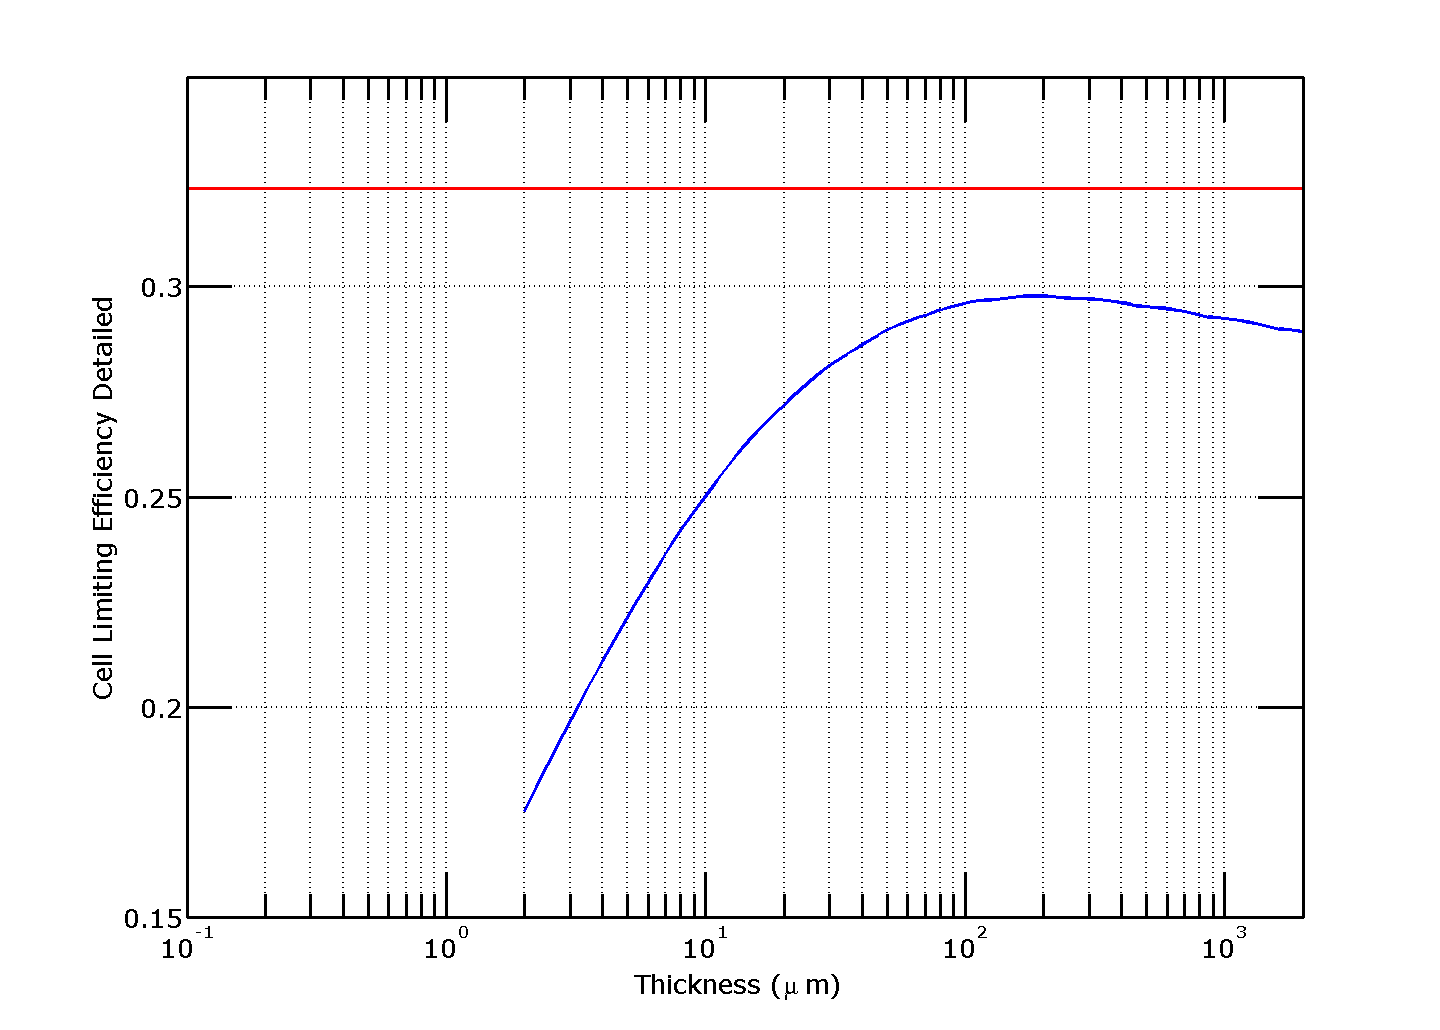
\includegraphics[width=0.45\textwidth]{Figures/LimitingEfficiencyDetailedVersusThickness}} 
 \caption[Detailed limiting efficiency versus thickness]{Limiting efficiency considering radiative recombination, Auger recombination, and free carrier absorption versus thickness for silicon.}
  \label{fig:limitingEfficiencyVersusThickness}
\end{figure}

One approach to \textbf{light trapping} is to use roughened surfaces which scatter or randomize the light upon reflection.  This geometrical optics light trapping limit is often referred to as the Yablonovitch limit\cite{Yablonovitch:82july} or the Lambertian limit, because Lambertian surfaces may be utilized to randomize light \cite{Sheng:84}.  The mean path length of light inside the material may be increased from $2 L$ to $4 n^2 L$ where $n$ is the index of refraction.  The absorption is 

\begin{equation}
A(E) = \frac{\alpha(E)}{\alpha(E) + \frac{1}{4 n^2 L}}
\end{equation}
For silicon, a 2 \hbox{\textmu}m film with light trapping may be enhanced to absorb light by about the same amount as that of a 50 \hbox{\textmu}m film.  

\begin{figure}[H]
\centering
\vspace{-10pt}
{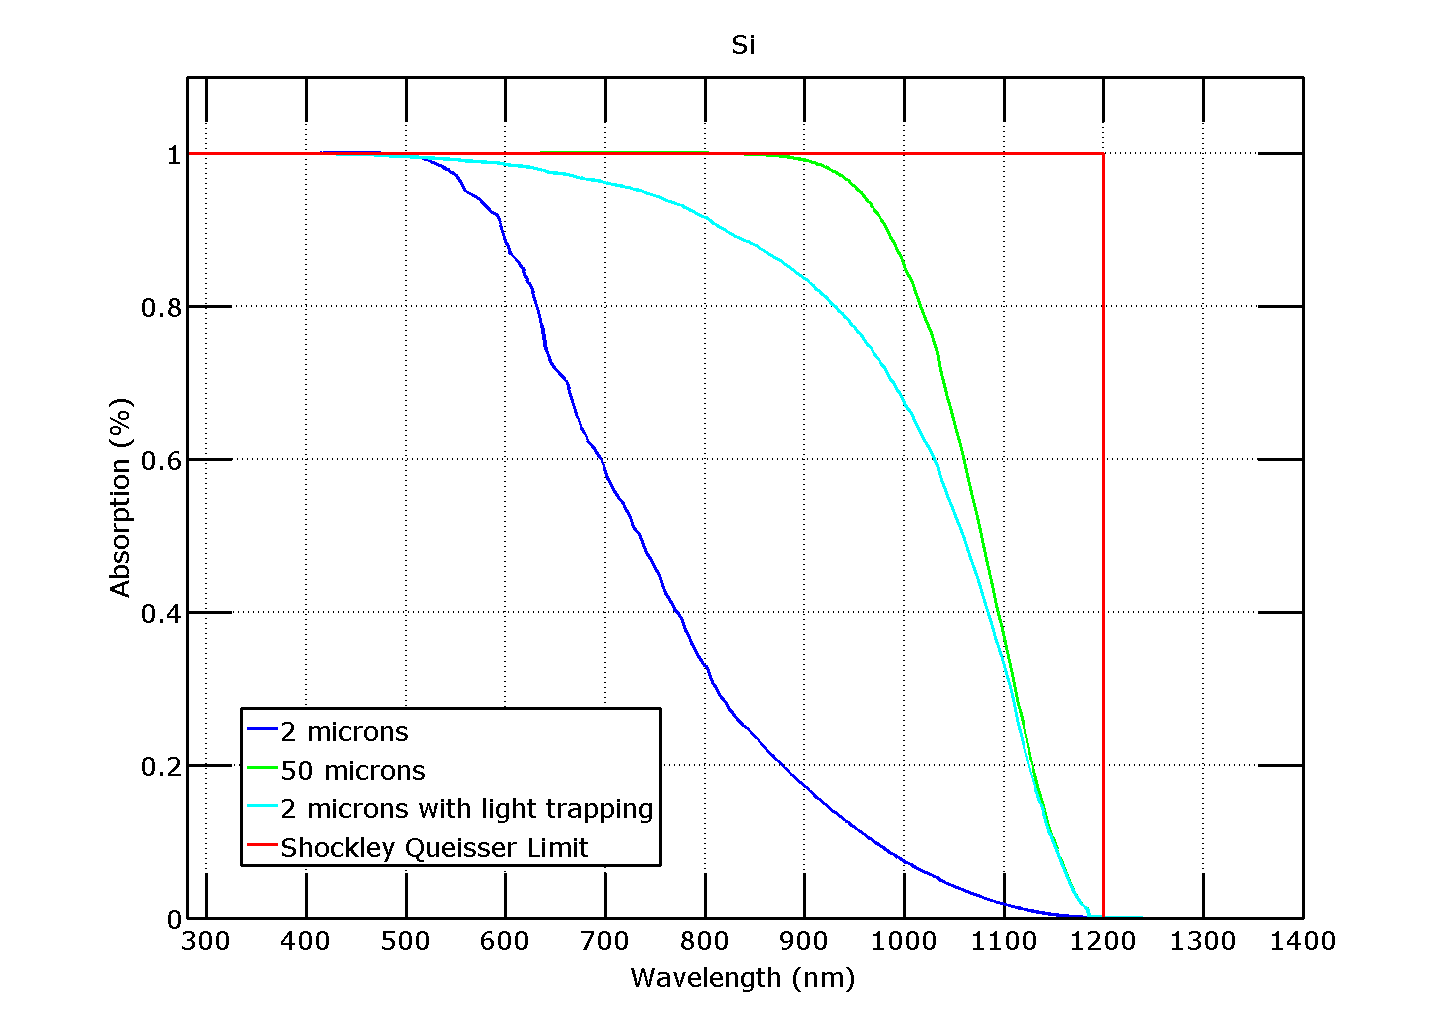
\includegraphics[width=0.45\textwidth]{Figures/SiliconFilmAbsorptionWLightTrappingVersusWavelength}} 
 \caption[Absorption with light trapping]{Using light trapping to enhance silicon thin film absorption.}
  \label{fig:limitingEfficiencyVersusThickness}
\end{figure}

The efficiencies are enhanced as can be seen in the plots below.  
\begin{figure}[H]
\centering
\vspace{-10pt}
{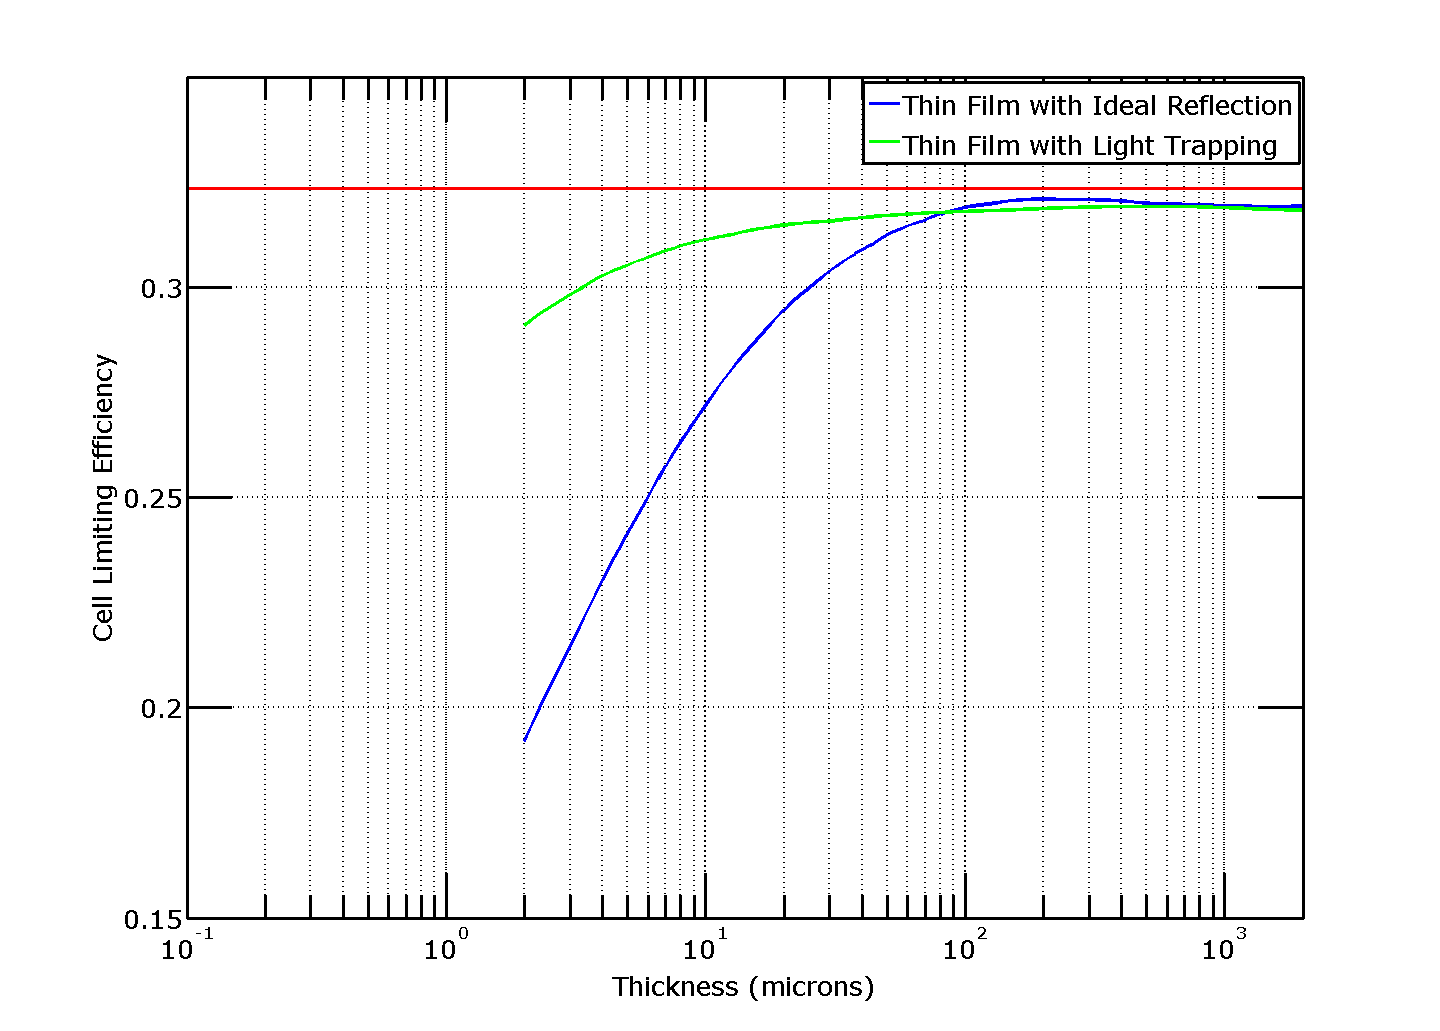
\includegraphics[width=0.45\textwidth]{Figures/LimitingEfficiencyVersusThicknessWLambertian}} 
 \caption[Limiting efficiency with light trapping]{Using light trapping to enhance silicon thin film limiting efficiency.}
  \label{fig:limitingEfficiencyVersusThickness}
\end{figure}

The ideal efficiency is 30.8\% at a thickness of about $L = 40$ \hbox{\textmu}m.
\begin{figure}[H]
\centering
\vspace{-10pt}
{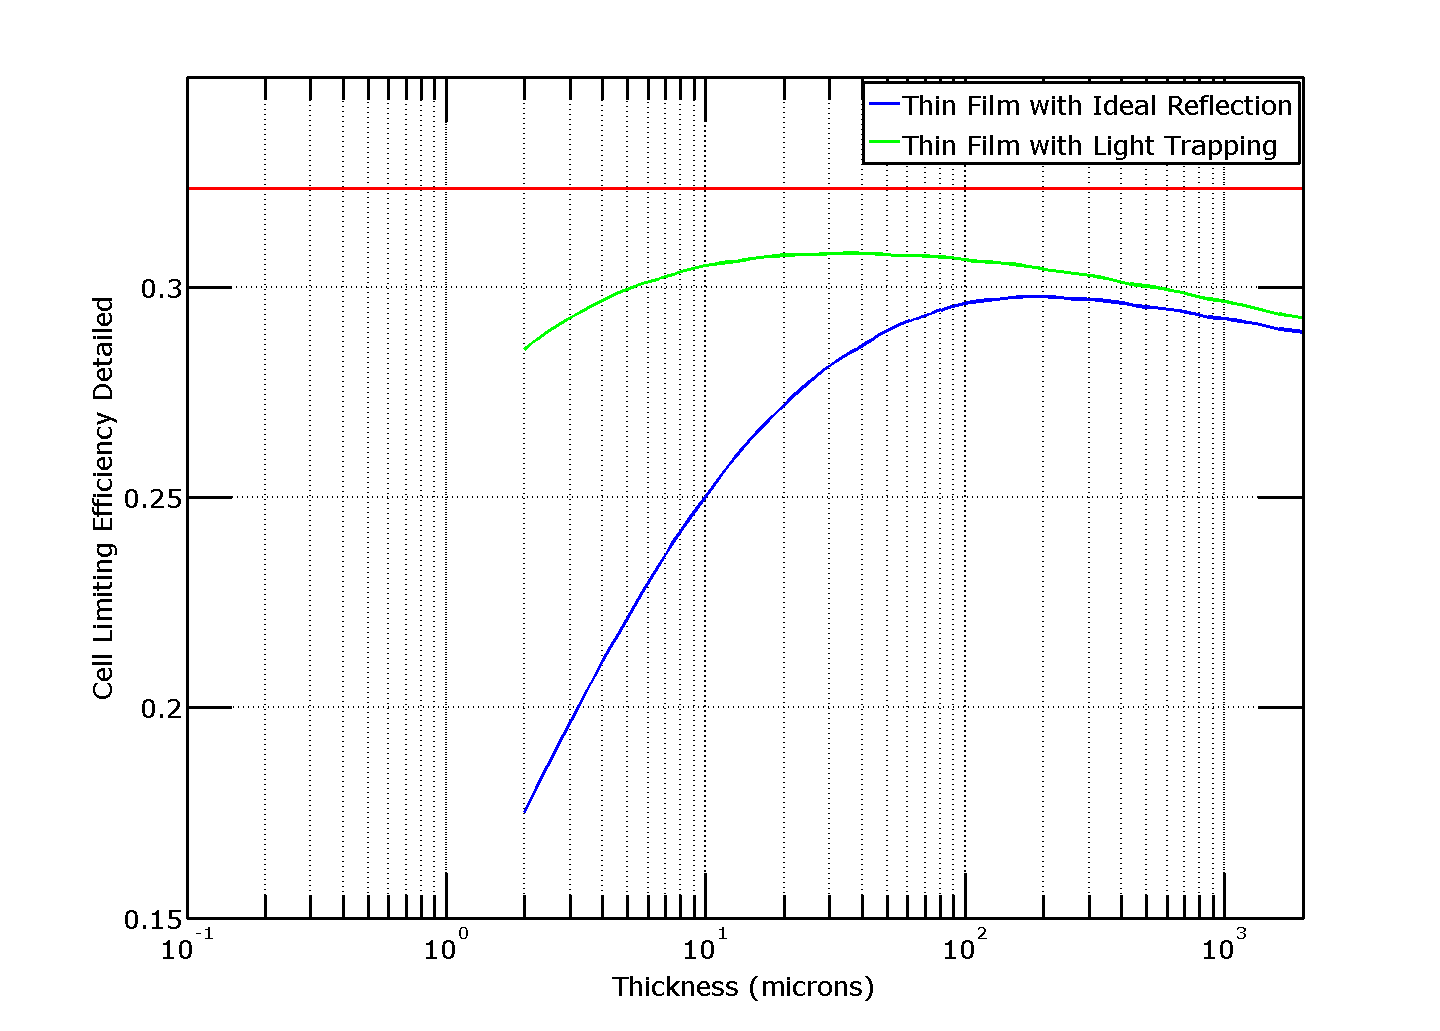
\includegraphics[width=0.45\textwidth]{Figures/LimitingEfficiencyDetailedVersusThicknessWLambertian}} 
 \caption[Detailed limiting efficiency with light trapping]{Using light trapping to enhance silicon thin film detailed limiting efficiency.}
  \label{fig:limitingEfficiencyVersusThickness}
\end{figure} 

\section{Transverse Modes}

The \textbf{plane of incidence} is is defined as the plane spanned by the incident plane wave, reflected propagation wave, and transmission propagation wave.  It is also the plane spanned by the surface normal and the incident plane wave.  

Transverse modes are where a particular field is transverse to the plane of incidence.  
The \textbf{TE mode} (Transverse Electric) or s wave is where the electric field $\textbf{E}$ is transverse to the plane of incidence.  The \textbf{TM mode} is where the magnetic field vector $\textbf{M}$ is transverse to the plane of incidence.  

\section{Transfer Matrix Method for Isotropic Layered Media}

\subsection{$2 \times 2$ Matrix Formulation for a Thin Film}

For reflection and transmission of electromagnetic radiation through a thin film using a $2 \times 2$ matrix method, 
\begin{equation}
n(\nu, x) = \begin{cases} 
n_1, x < 0 \\
n_2, 0 < x < d, \\
n_3, d < x
\end{cases} 
\end{equation}
where $n_1$, $n_2$, and $n_3$ are the refractive indices and $d$ is the thickness of the film.  
The electric field that satisfies Maxwell's equations has the form
\begin{equation}
E = E(x) e^{i (\omega t - \beta z)}
\end{equation}
where $\beta$ is the $z$ component of the wave vector and $\omega$ is the angular frequency.  
The electric field consists of a right-traveling wave and a left-traveling wave and can be written as 
%\begin{equation}
%
%\end{equation}

This material is largely taken from Chapter 5 of Reference \cite{Yeh:05}.  
The transfer matrix method is a powerful approach for solving the propagation of electromagnetic radiation through a multilayer system.  
The multilayer system is comprised of $N$ layers of materials with $d_i$ thicknesses and 

\begin{equation}
n(\nu, x) = \begin{cases} 
n_0(\nu), x < x_0, \\
n_1(\nu), x_0 < x < x_1, \\
n_2(\nu), x_1 < x < x_2 ,\\
\hspace{1em} \vdots \hspace{4em} \vdots \\
n_N(\nu), x_{N-1} < x < x_N, \\
n_{N+1}(\nu), x_N < x
\end{cases} 
\end{equation}
where $n_l$ is the refraction index of the $l$th layer, $x_l$ is the position of the interface between the $l$th layer and the $(l+1)$th layer, $n_0$ is the index of refraction of the incident medium, and $n_{N+1}$ is that of the transmitted wave.  

The layer thicknesses $d_l$ are related to the $x_l$'s by 
\begin{equation}
\begin{aligned}
d_1 &= x_1 - x_0, \\
d_2 &= x_2 - x_1, \\
& \vdots  \\
d_N &= x_N - x_{N-1} 
\end{aligned}
\end{equation}

The electric field of a general plane-wave solution can be written as 
\begin{equation}
E = E(x) e^{i (\omega t - \beta z)}
\end{equation}
where the electric field distribution $E(x)$ can be written as 
\begin{equation}
E(x) = \begin{cases}
A_0 e^{-i k_{0x} (x - x_0)} + B_0 e^{i k_{0x} (x - x_0)}, x < x_0 \\
A_l e^{-i k_{lx} (x - x_0)} + B_l e^{i k_{l x} (x - x_0)}, x_{l-1} < x < x_l \\
A_{N+1} e^{-i k_{0x} (x - x_0)} + B_{N+1} e^{i k_{0x} (x - x_0)}, x_{N} < x \\
\end{cases}
\end{equation}
where $k_{lx}$ is the $x$ component of the wave vectors
\begin{equation}
k_{lx} = \left [ \left ( n_l \frac{\omega}{c} \right ) ^2 - \beta^2 \right ] ^{1/2}, l = 0, 1, 2, \ldots N, N+1
\end{equation}
and is related to the ray angle $\theta_l$ by
\begin{equation}
k_{lx} = n_l \frac{\omega}{c} \cos \theta_l.  
\end{equation}
Using the same argument as in 



\bibliographystyle{IEEEtran}
\bibliography{AllRefs}

\end{document}

